%\newpage
\subsection{Оперативное планирование производства}
\label{bp:OperPlan}

Оперативным планированием производства занимается отдел планирования производства. 

Состав отдела планирования на момент проведения аудита: начальник отдела, старший специалист по планированию производства, специалист по планированию производства. График работы 5/2.

Планирование происходит в системе 1С: УПП, обработка ''Рабочее место планирование гофротара'' (рис. \ref{pic:VII 12}).


Специалист по планированию производства в начале рабочего дня в системе 1С: УПП формирует отчет ''Загрузка оборудования по датам (план) по заданиям на производство'' (рис. \ref{pic:ПЛ1}). Структура отчета - дерево с группировками по каждой линии в отдельности (рис. \ref{pic:ПЛ2}). 

Отставание или опережение корректируется в ручную, при этом отставание добавить на ЛГК в текущие сутки программа не позволяет, специалист рассчитывает отставание по времени и это отставание корректирует (убирает раскрои из действующих суток).

Специалист по планированию на опыте или по согласованию с технологическим отделом может поменять маршрут изготовления, внеся изменения в документ ''Заказ на производство'' (рис. \ref{pic:ПЛ3} - \ref{pic:ПЛ4}).

При завершении выполнения заказа на основании отчета ''Отчет Анализ предварительных заявок'' (рис. \ref{pic:ПЛ5}) специалист по планированию в отчете выделяет нужную строку в табличной части и применяет команду ''Завершить заказ на производство'' (рис. \ref{pic:ПЛ6}). 

После того как все линии переработки скорректированы, специалист начинает планирует раскрои на ГА.
Для этого специалист открывает форму ''Помощник планирования раскроев гофротары (гофроагрегат)'' (рис. \ref{pic:ПЛ7}), в которой вручную формирует раскрои с помощью перебирания позиций и расчетов, производимых на калькуляторе. 

Горизонт планирования ГА и линий переработки не ограничен, все зависит от количества невыполненных производством заказов. Возможность внесения изменений в композиционный состав представлена на рис. \ref{pic:ПЛ8} - \ref{pic:ПЛ10}, вносить изменения в справочник композиций специалист по планированию не может.

Сменные задания на ГА формируются из расчета на 12 часов работы (рис. \ref{pic:ПЛ11}). 
Задания на ГА и на ПЛ распечатывается и передается в производство (рис. \ref{pic:ПЛ12}). После того как план на ГА сформирован, специалист по планированию приступает к планированию ПЛ (рис. \ref{pic:ПЛ14}), при этом не производится сверка по простоям (рис. \ref{pic:ПЛ13}). Сформированное сменное задание выводится на печать и передается на производство.
Менеджер по логистике

Каждый день отдел планирования в 10-00 и в 15-00 выгружает из 1С: УПП ''План отгрузки'', подтверждает  либо не подтверждает готовность тех или иных заказов в указанные сроки на определенную дату и отправляет это менеджеру по логистике.

При любом изменении, снятии, корректировке, сменные задания заново распечатываются и передаются на производство.


\clearpage




\begin{figure}
\begin{center}
 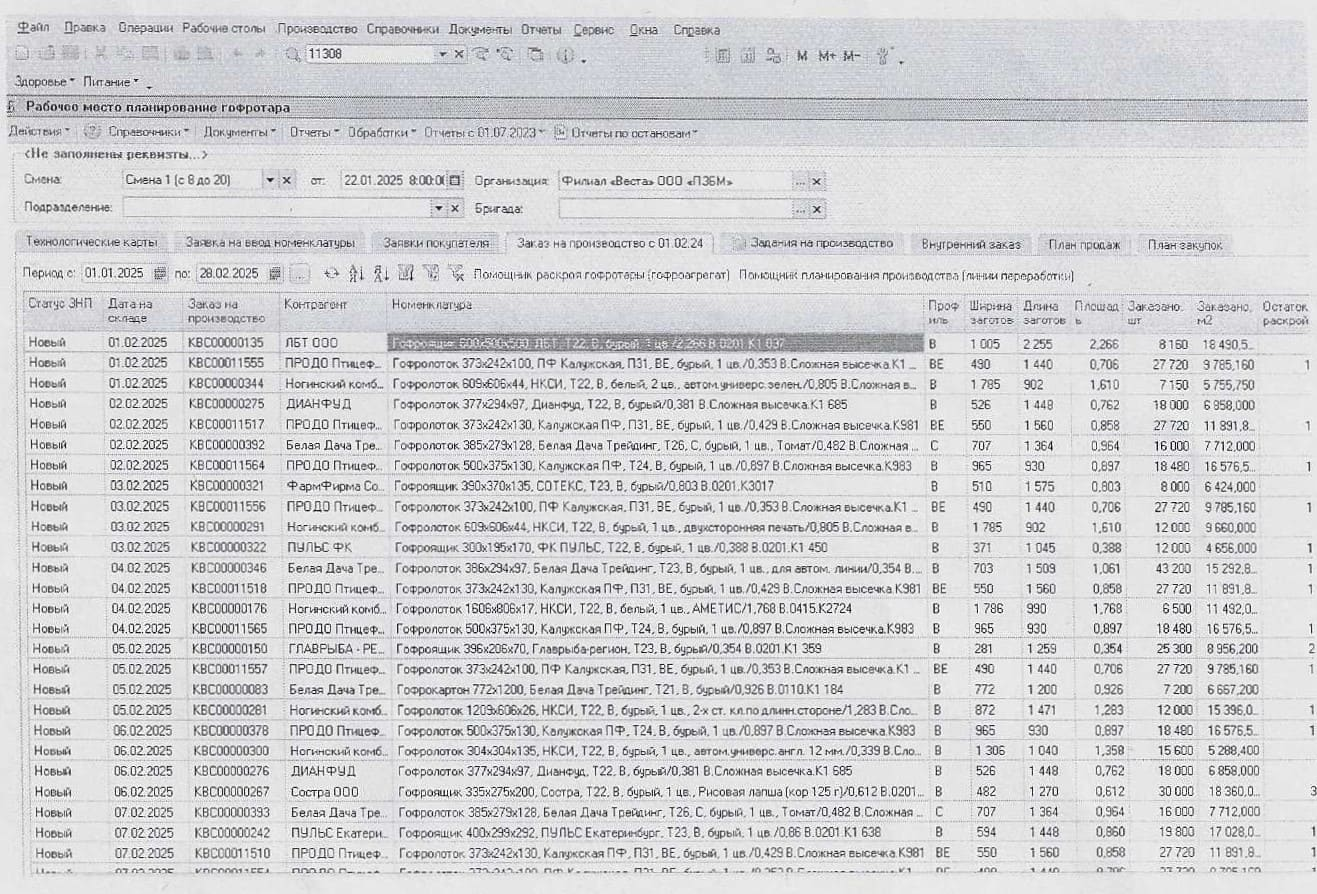
\includegraphics[height=0.4\textheight, keepaspectratio]{Pics/VII 12.jpg}
\end{center}
 \caption{Рабочее место планирование гофротара в 1С: УПП}
 \label{pic:VII 12}
\end{figure}



\begin{figure}
\begin{center}
 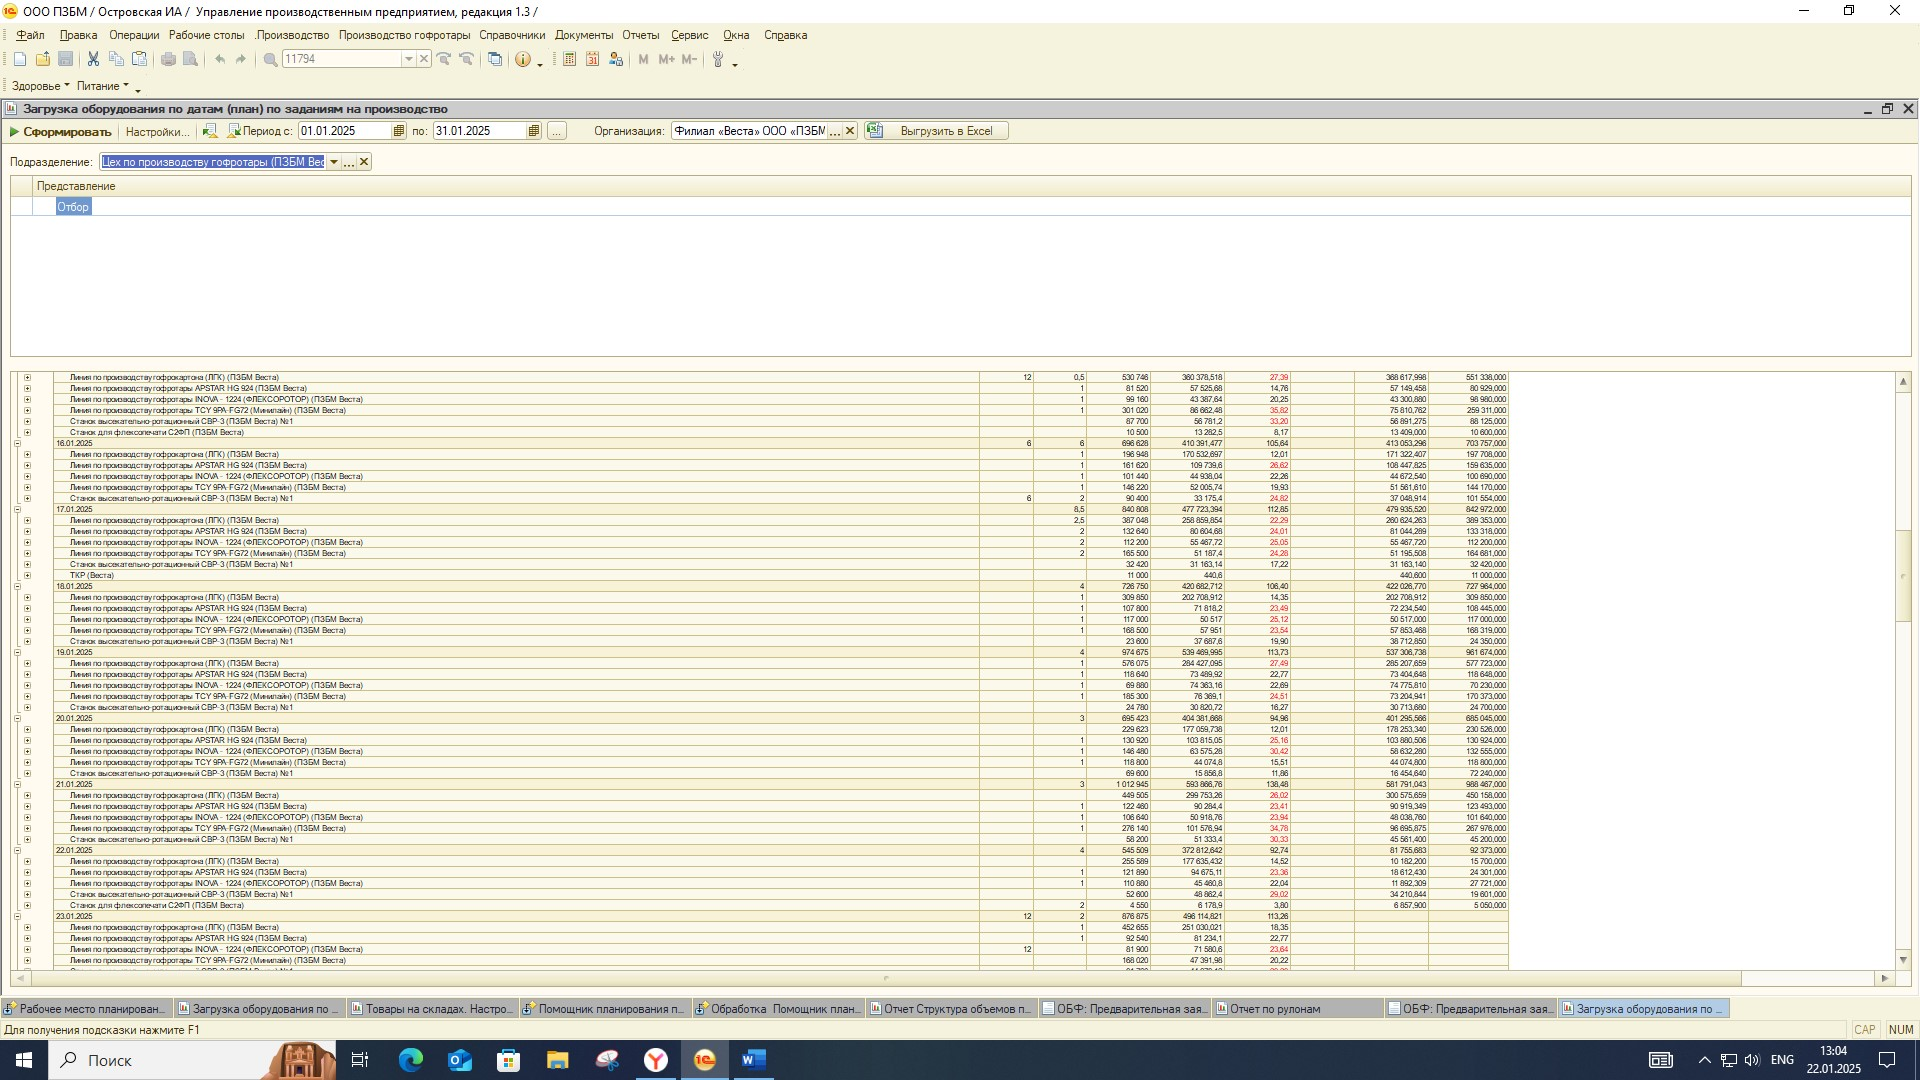
\includegraphics[height=0.35\textheight, keepaspectratio]{Pics/ПЛ1.jpg}
\end{center}
 \caption{Отчет Загрузка оборудования по датам (план) по заданиям на производство}
 \label{pic:ПЛ1}
\end{figure}


\begin{figure}
\begin{center}
 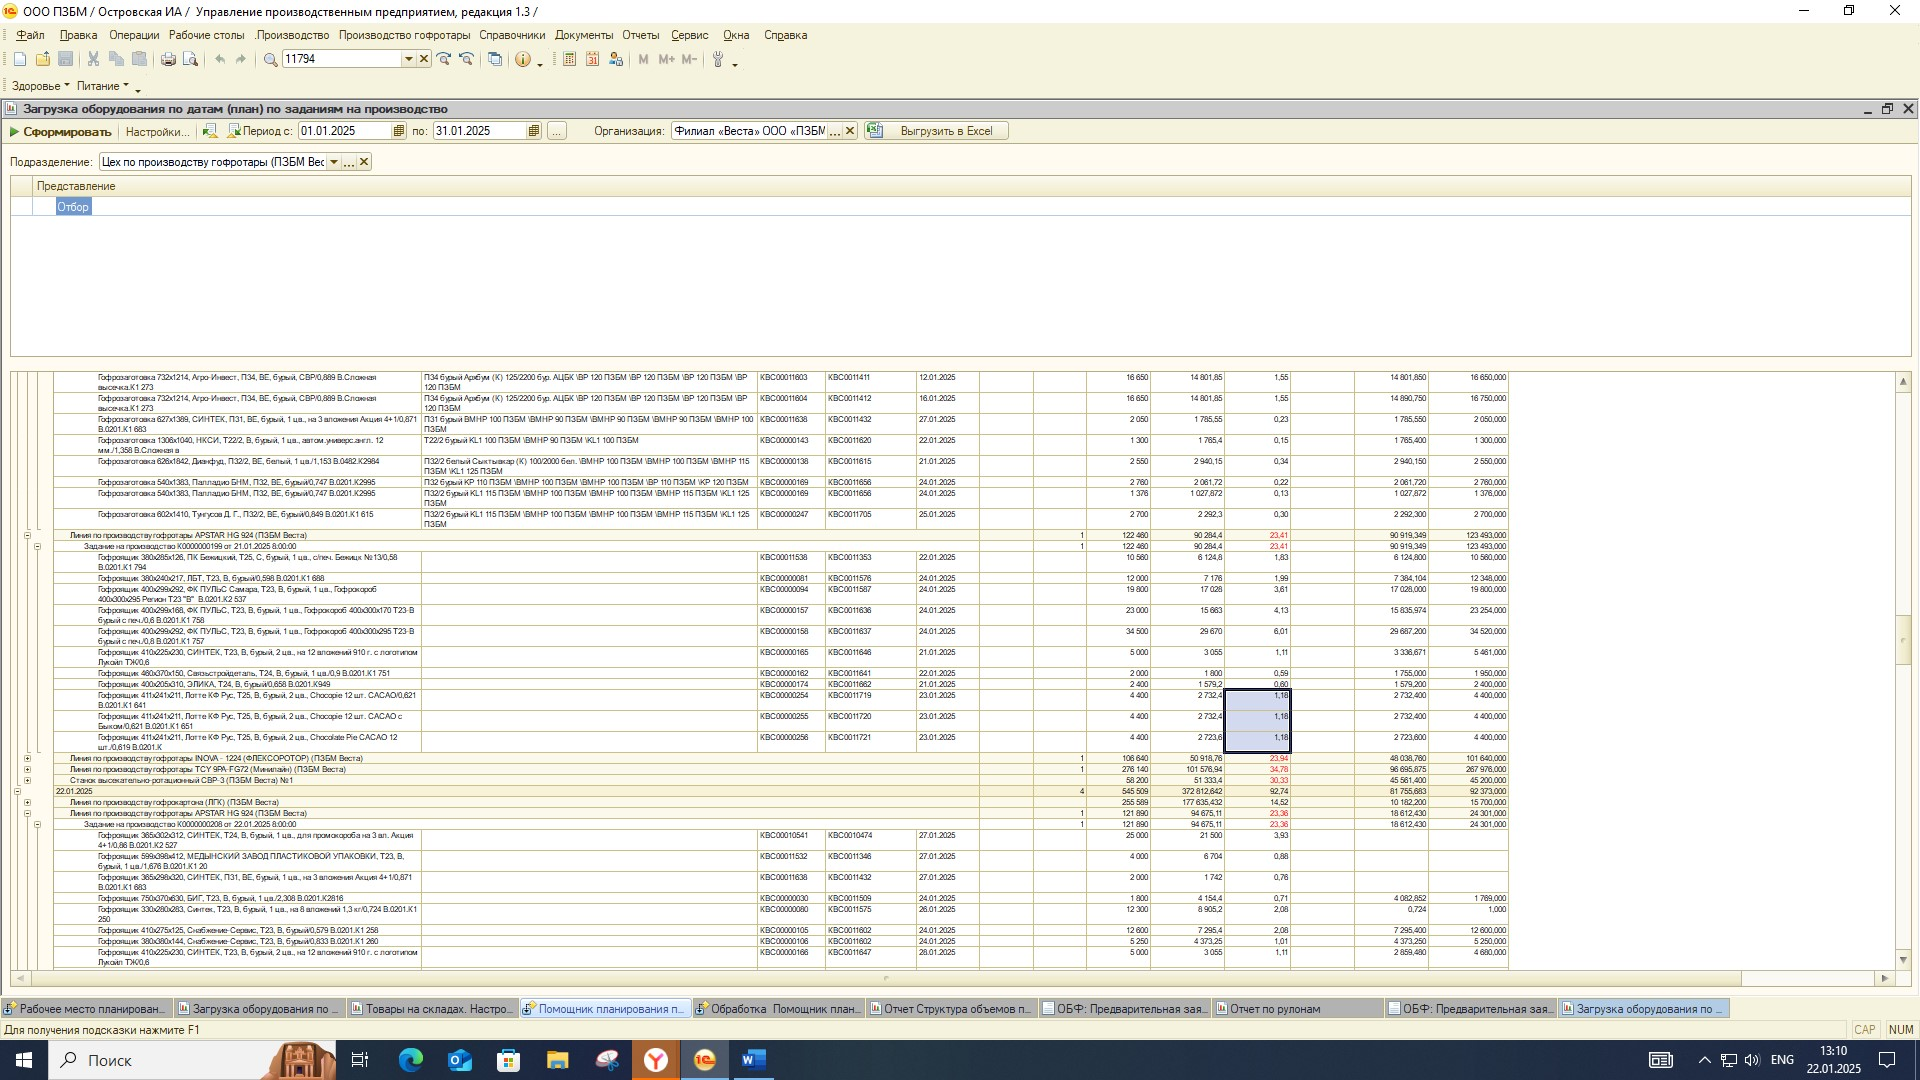
\includegraphics[height=0.45\textheight, angle=90, keepaspectratio]{Pics/ПЛ2.jpg}
\end{center}
 \caption{Отчет Загрузка оборудования по датам (план) по заданиям на производство-расширенный}
 \label{pic:ПЛ2}
\end{figure}


\begin{figure}
\begin{center}
 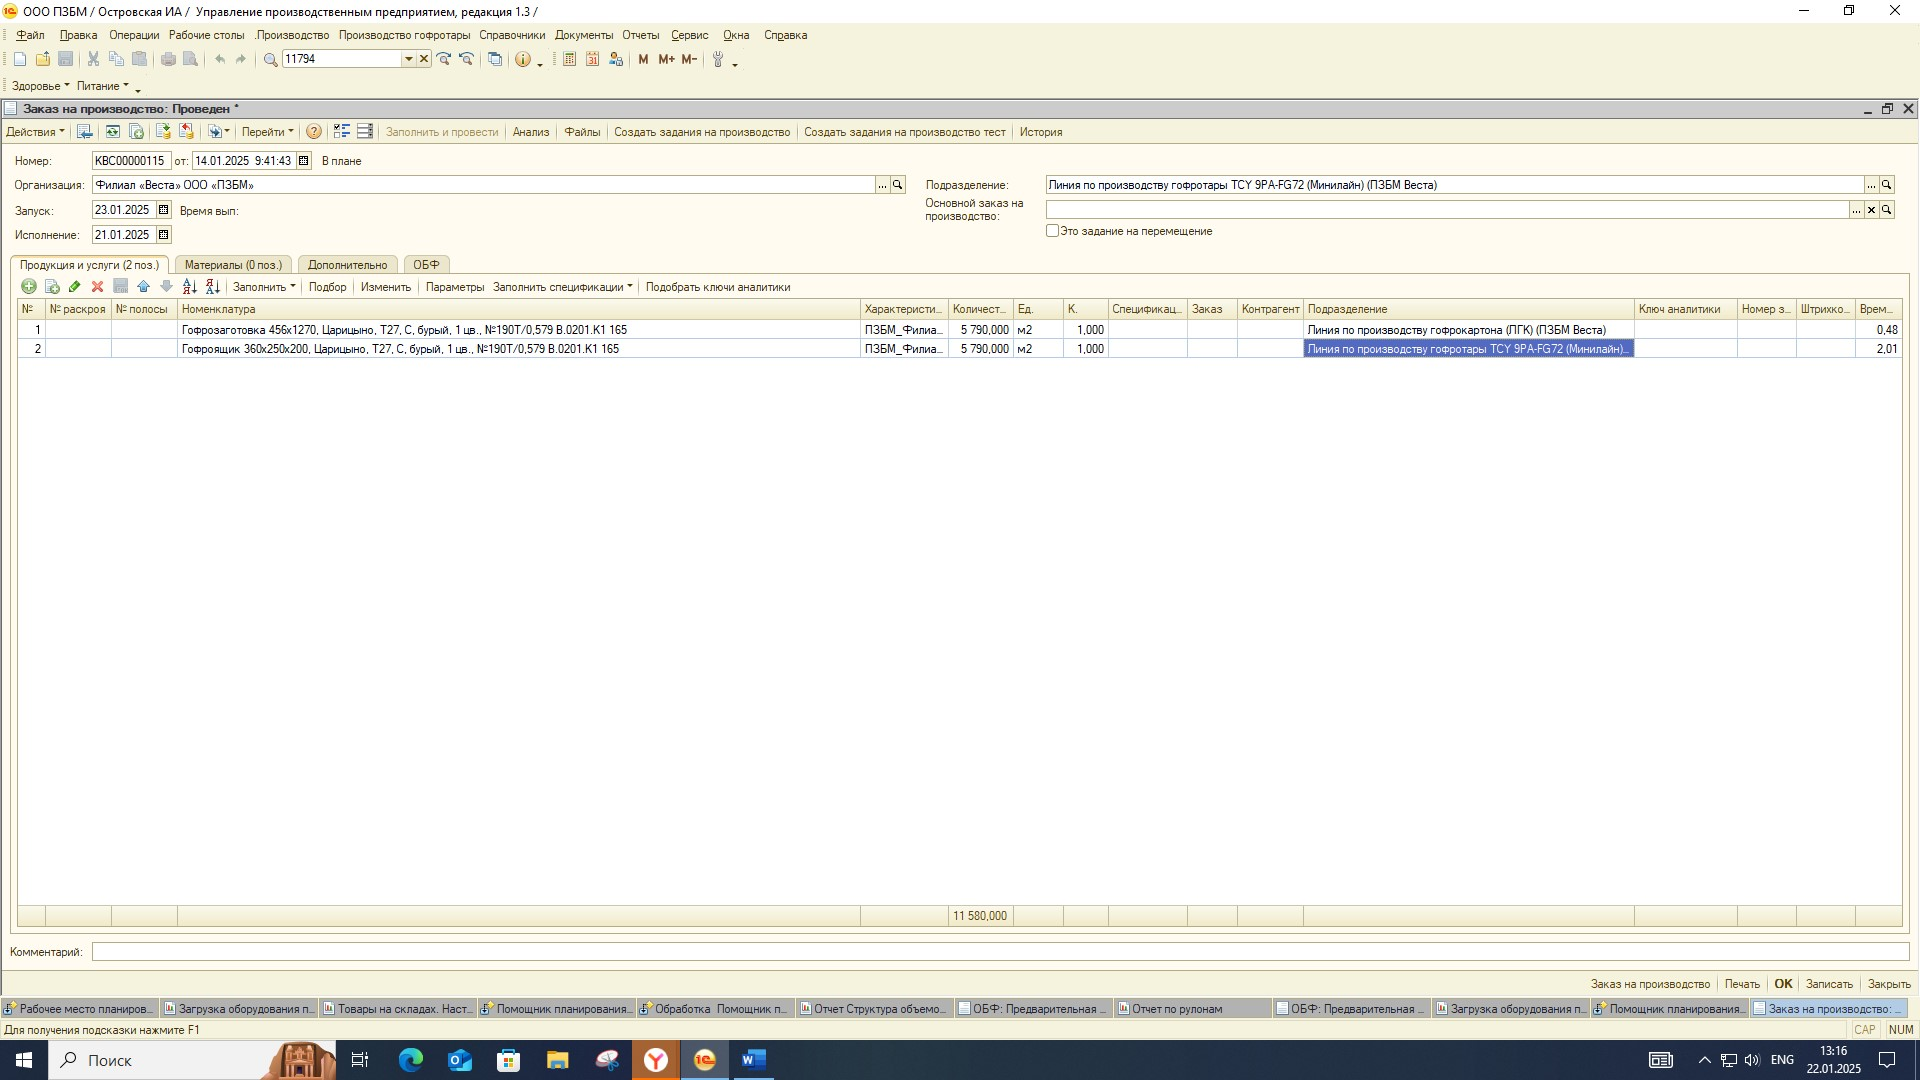
\includegraphics[height=0.35\textheight, keepaspectratio]{Pics/ПЛ3.jpg}
\end{center}
 \caption{Заказ на производство в 1С: УПП}
 \label{pic:ПЛ3}
\end{figure}


\begin{figure}
\begin{center}
 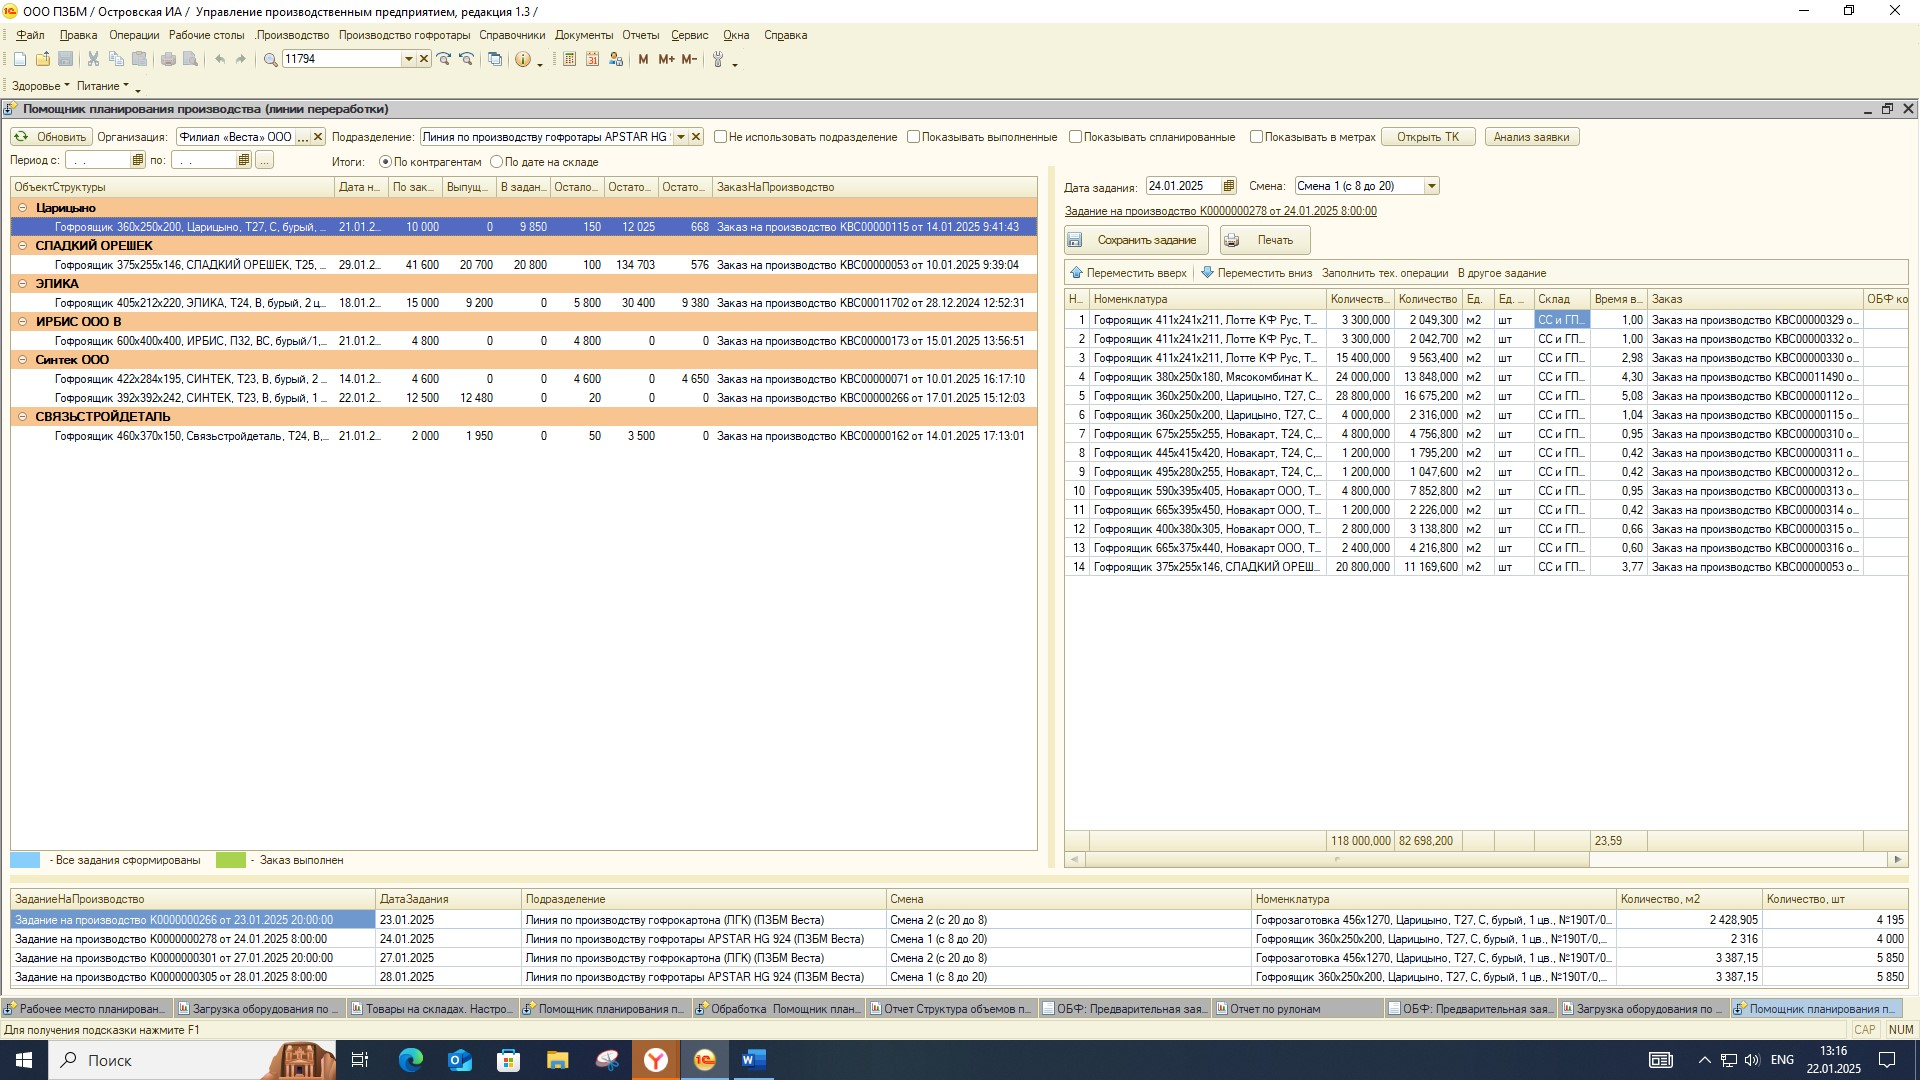
\includegraphics[height=0.35\textheight, keepaspectratio]{Pics/ПЛ4.jpg}
\end{center}
 \caption{Помощник планирования производства (линии переработки)}
 \label{pic:ПЛ4}
\end{figure}

\begin{figure}
\begin{center}
 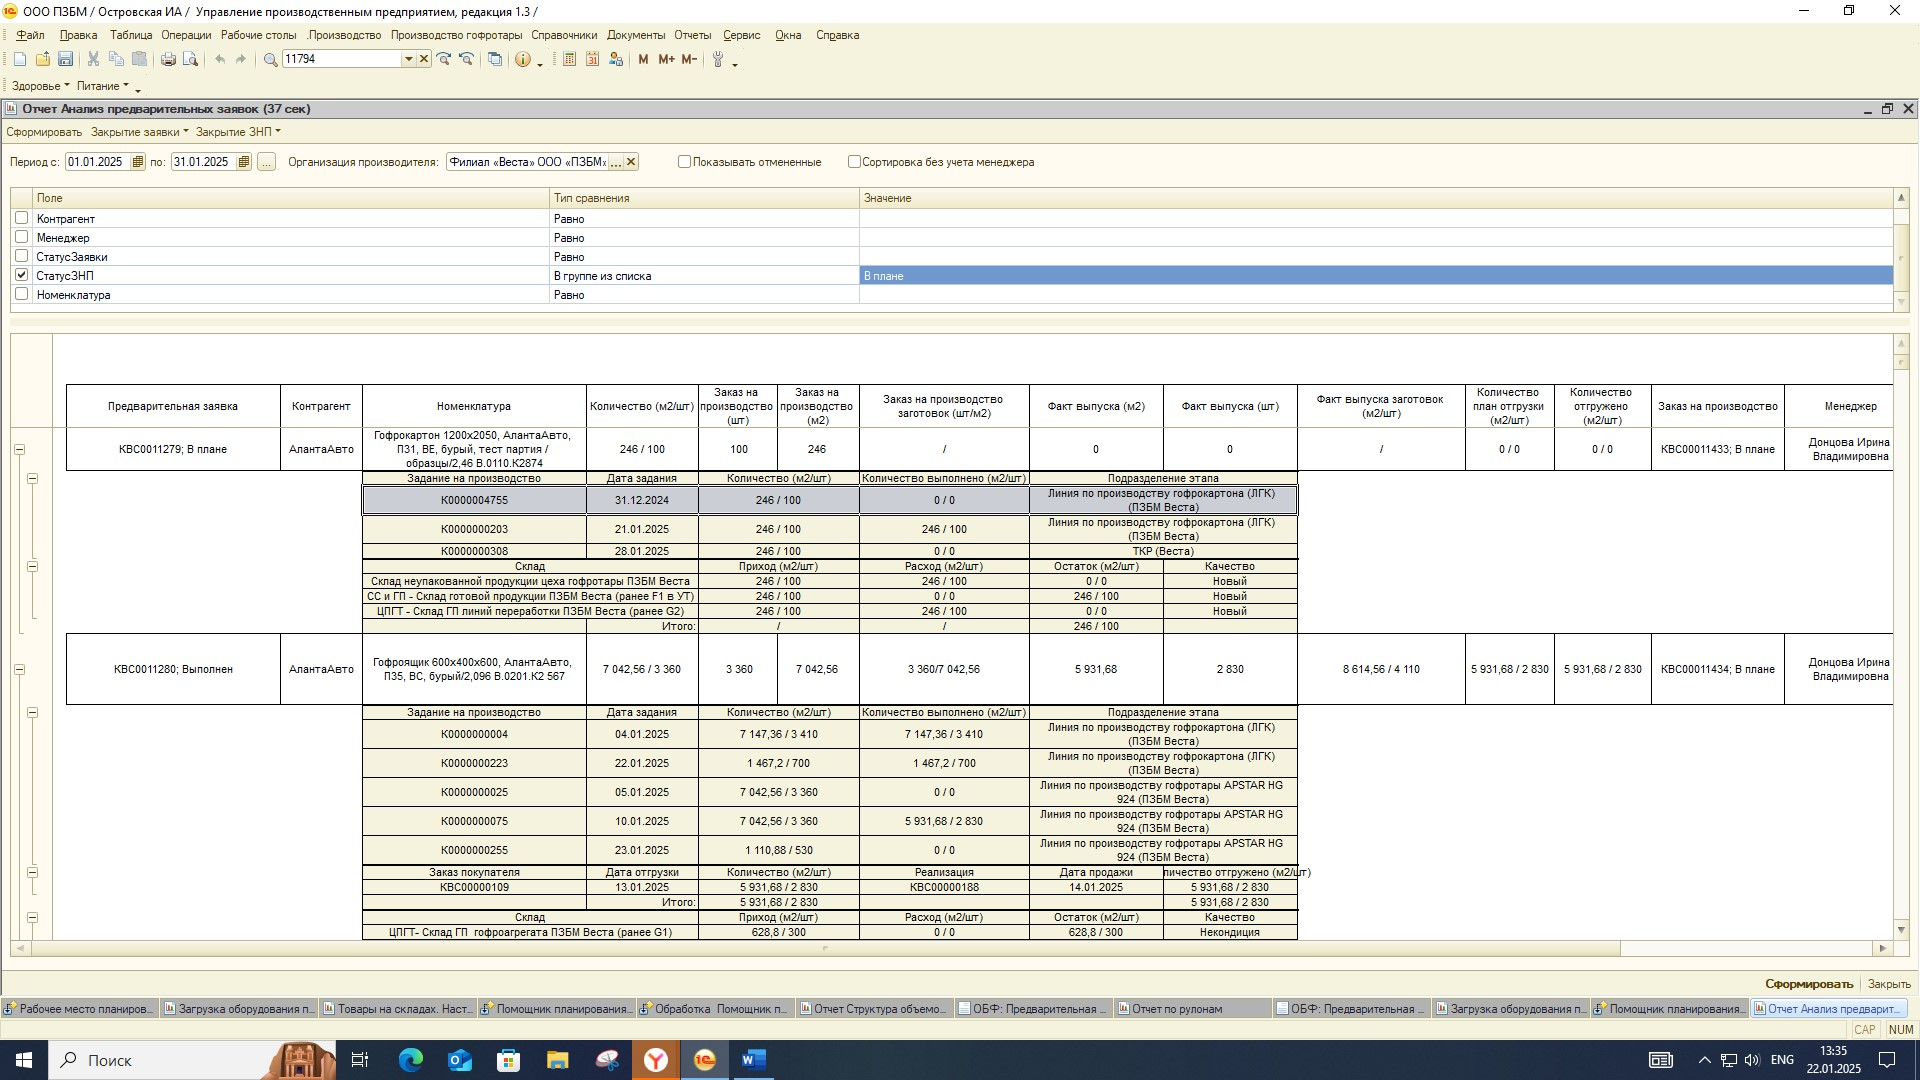
\includegraphics[height=0.35\textheight, keepaspectratio]{Pics/ПЛ5.jpg}
\end{center}
 \caption{Отчет Анализ предварительных заявок}
 \label{pic:ПЛ5}
\end{figure}

\begin{figure}
\begin{center}
 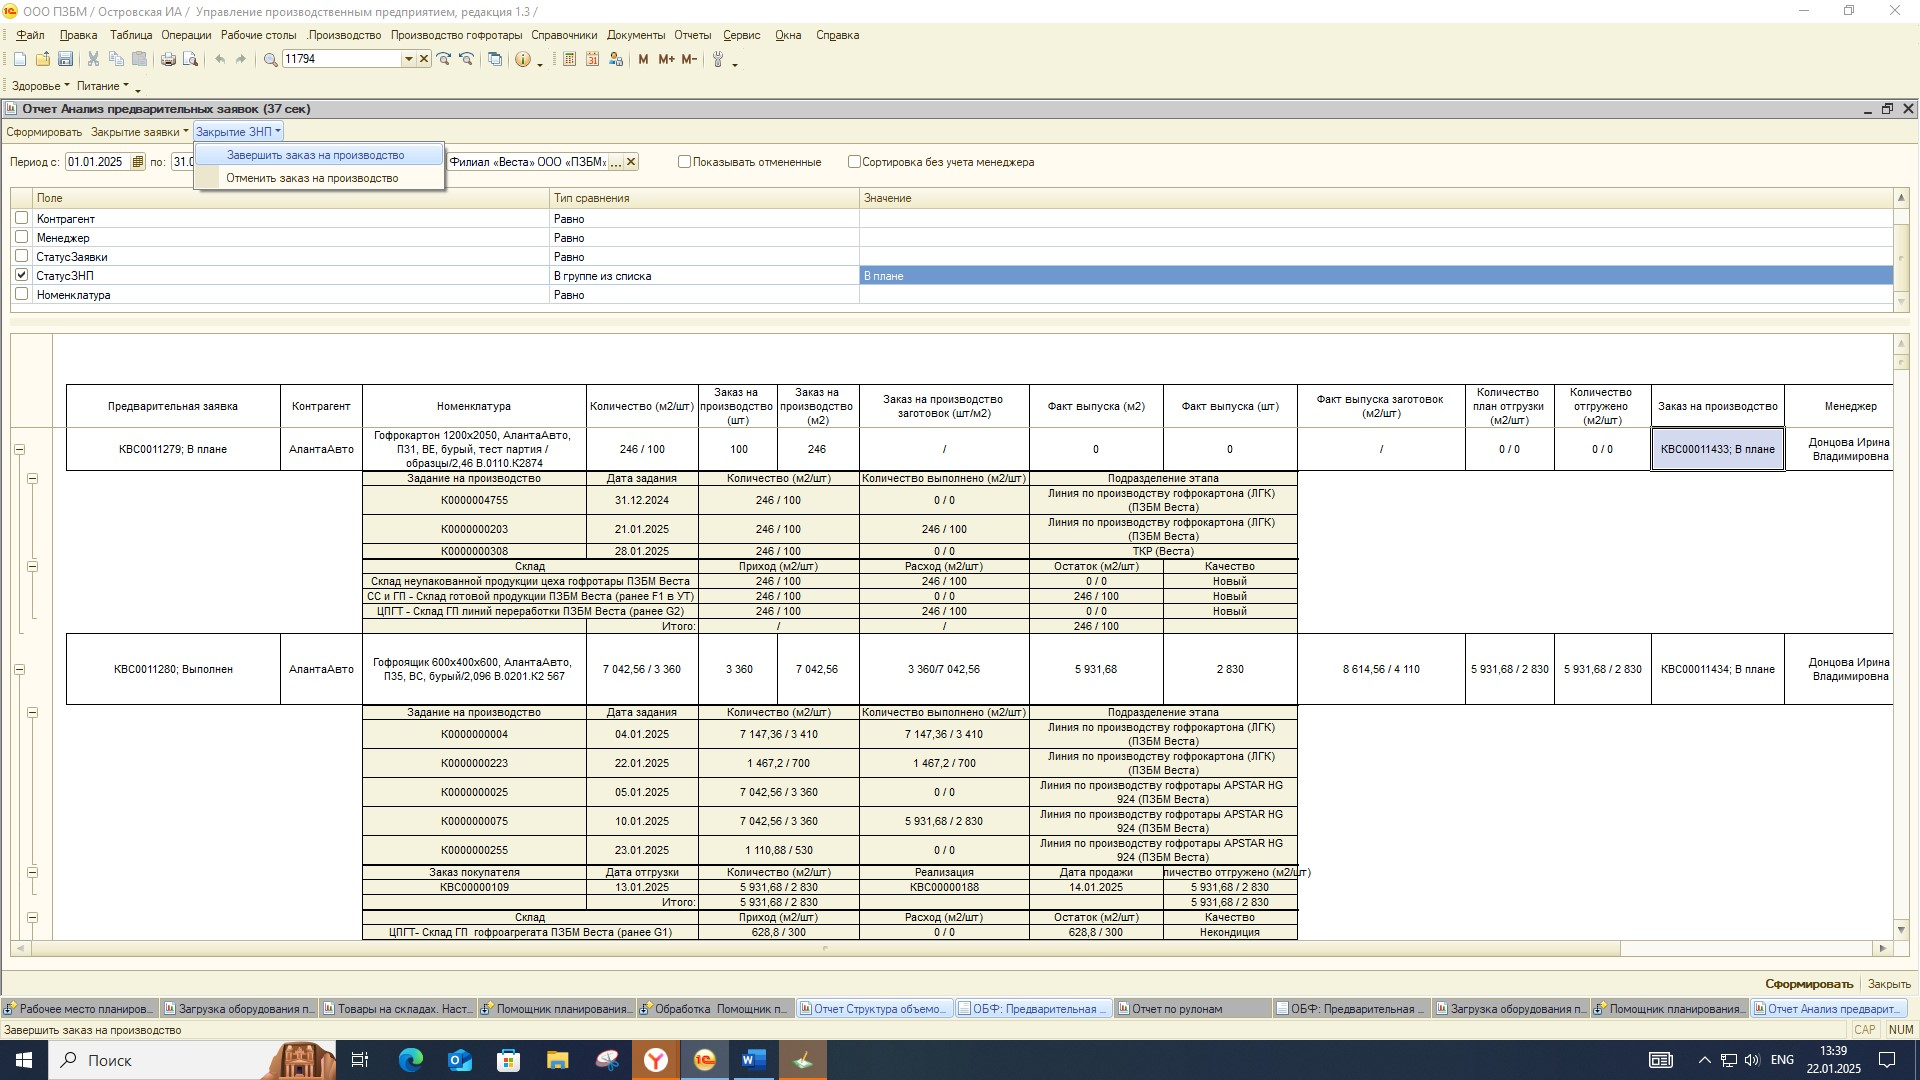
\includegraphics[height=0.35\textheight, keepaspectratio]{Pics/ПЛ6.jpg}
\end{center}
 \caption{Завершение заказа на производство}
 \label{pic:ПЛ6}
\end{figure}


\begin{figure}
\begin{center}
 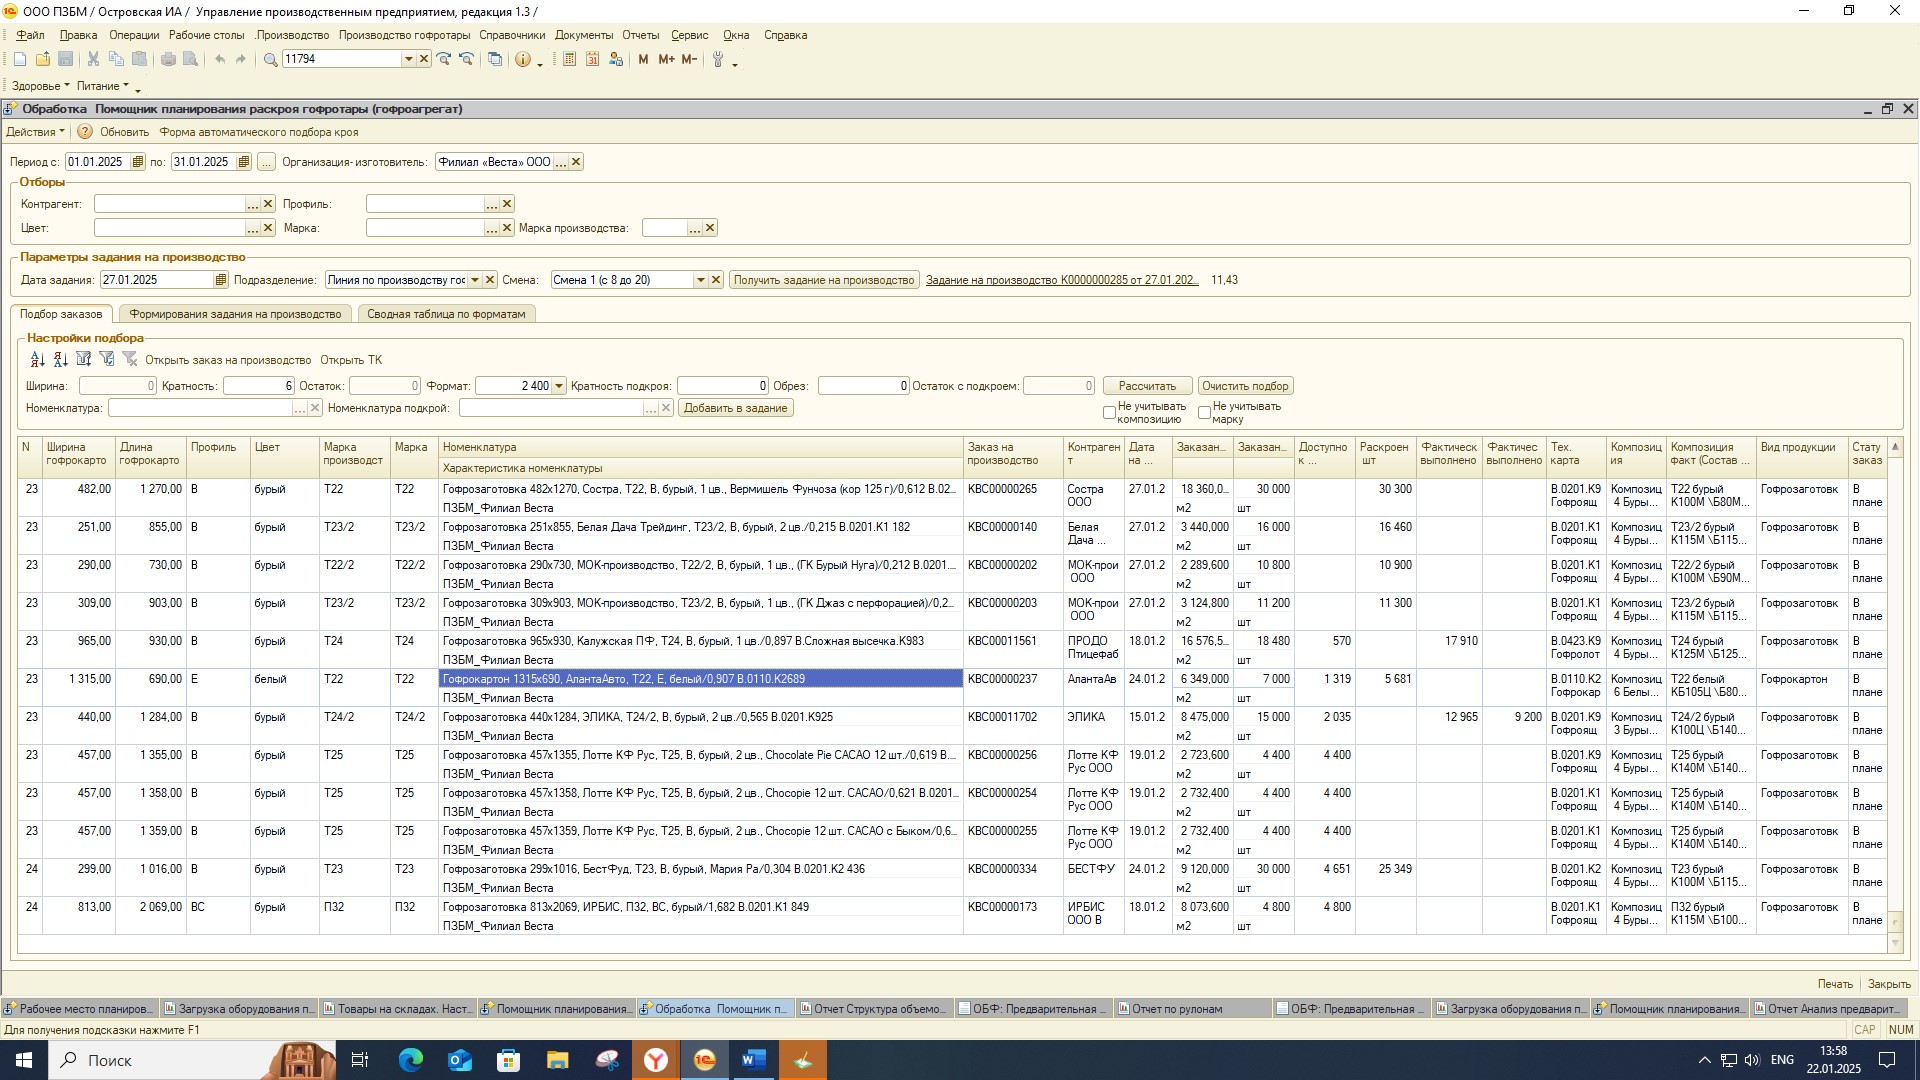
\includegraphics[height=0.45\textheight, angle=90, keepaspectratio]{Pics/ПЛ7.jpg}
\end{center}
 \caption{Помощник планирования раскроев гофротары (гофроагрегат)}
 \label{pic:ПЛ7}
\end{figure}


\begin{figure}
\begin{center}
 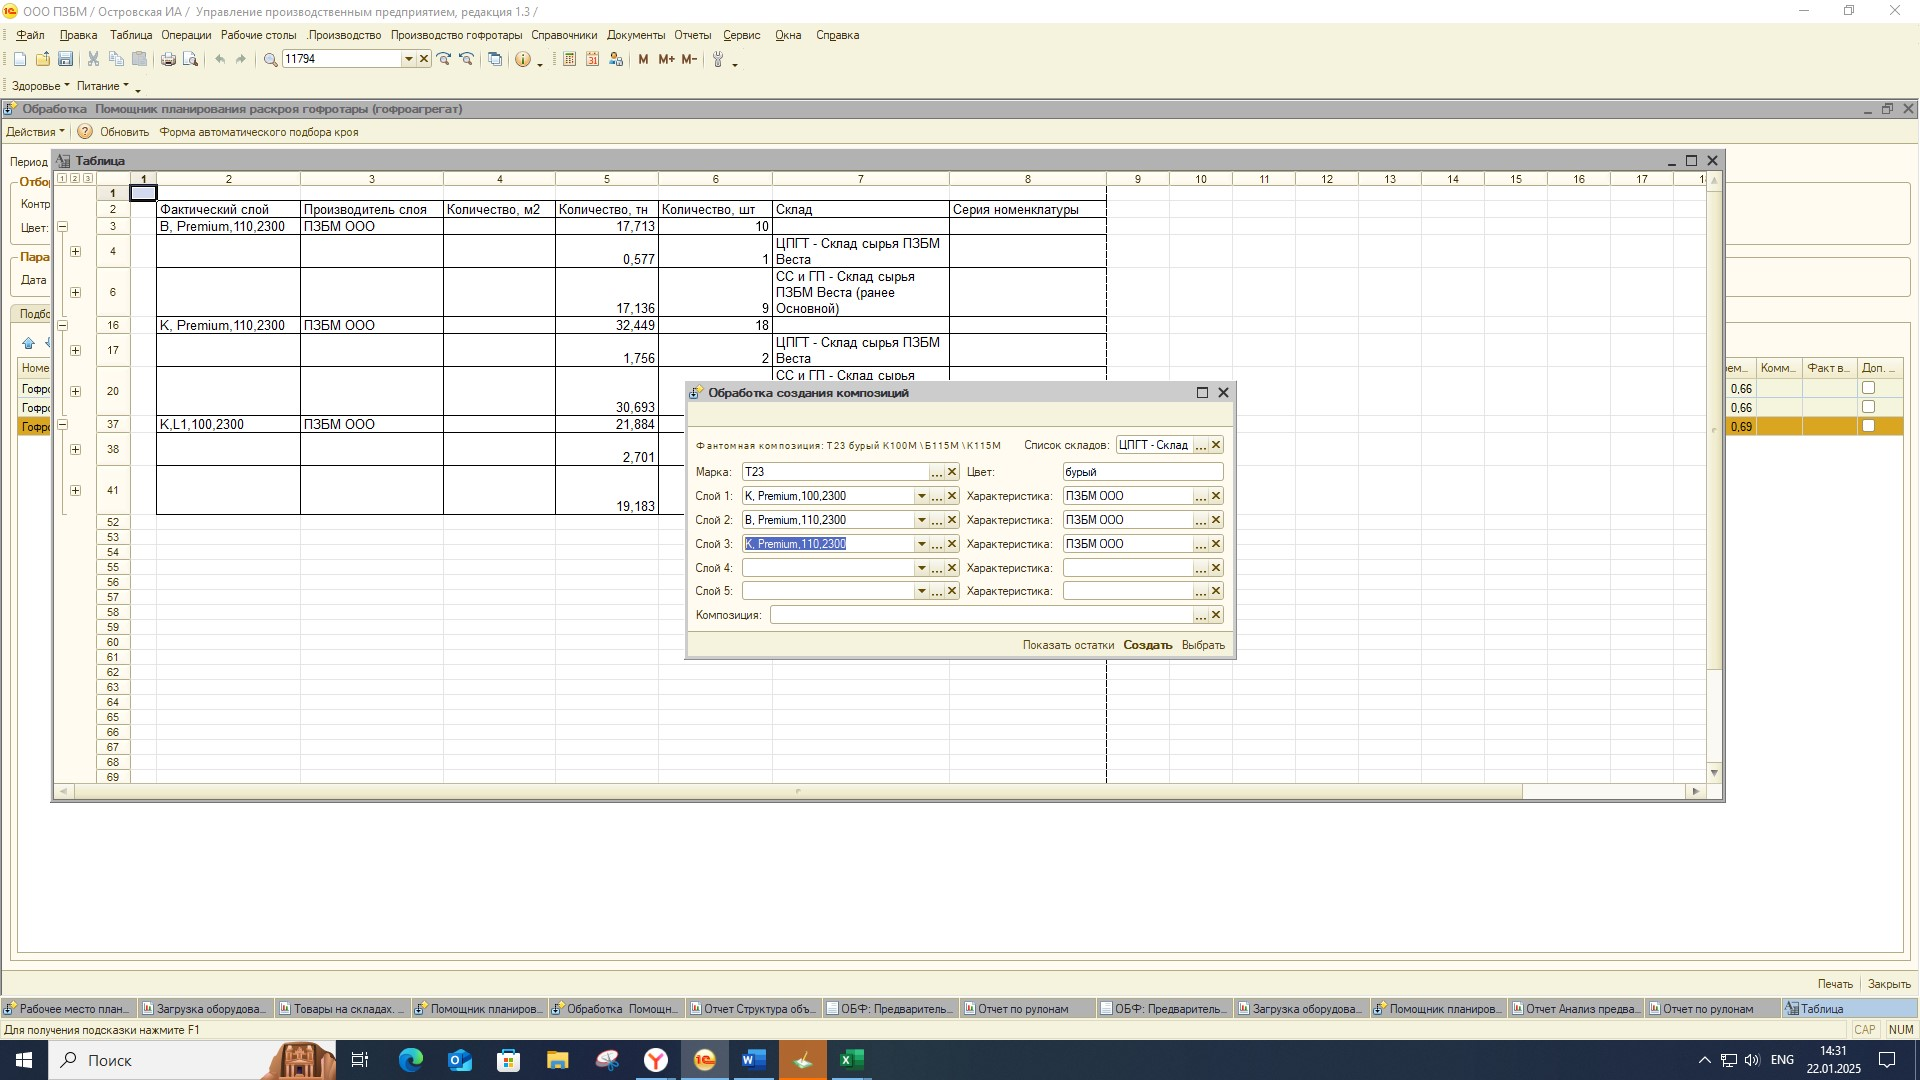
\includegraphics[height=0.35\textheight, keepaspectratio]{Pics/ПЛ8.jpg}
\end{center}
 \caption{Изменение композиции в раскрое}
 \label{pic:ПЛ8}
\end{figure}

\begin{figure}
\begin{center}
 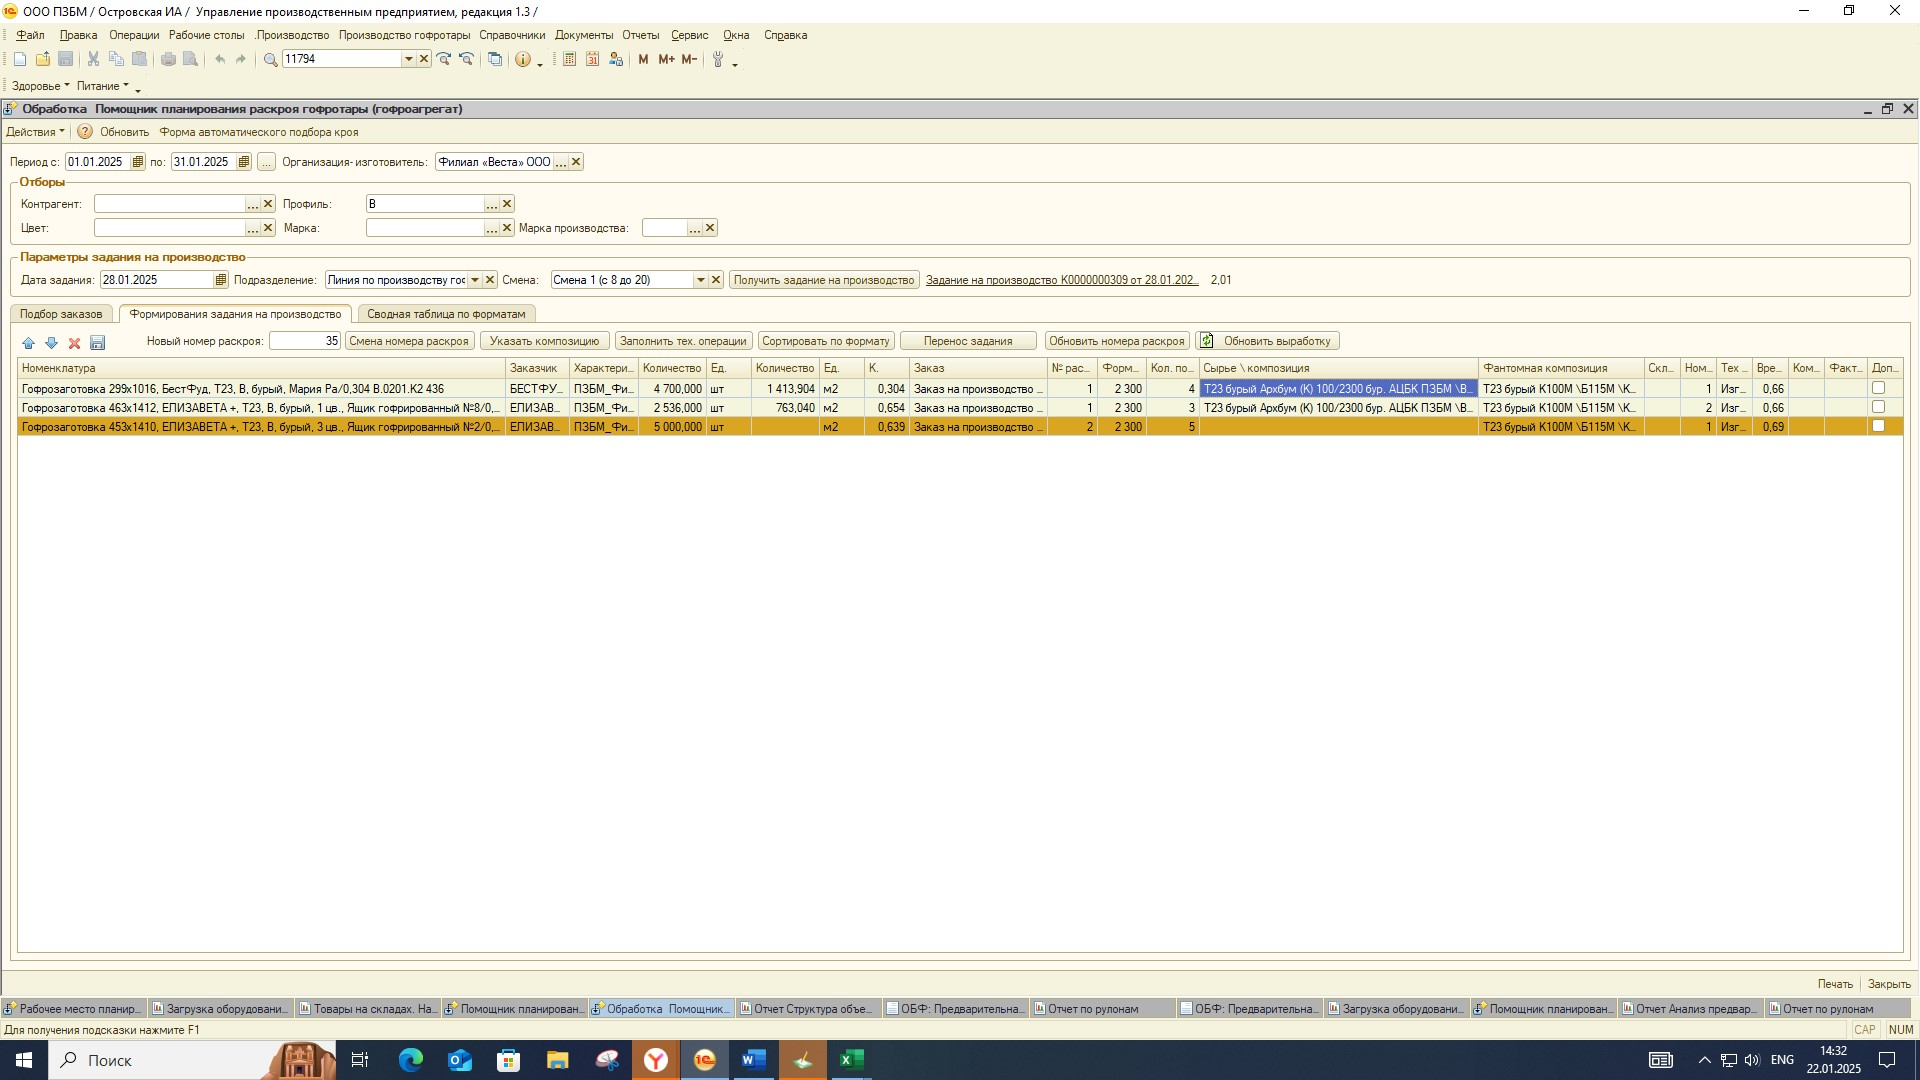
\includegraphics[height=0.35\textheight, keepaspectratio]{Pics/ПЛ9.jpg}
\end{center}
 \caption{Выбор раскроя для изменения номенклатуры в композиции}
 \label{pic:ПЛ9}
\end{figure}


\begin{figure}
\begin{center}
 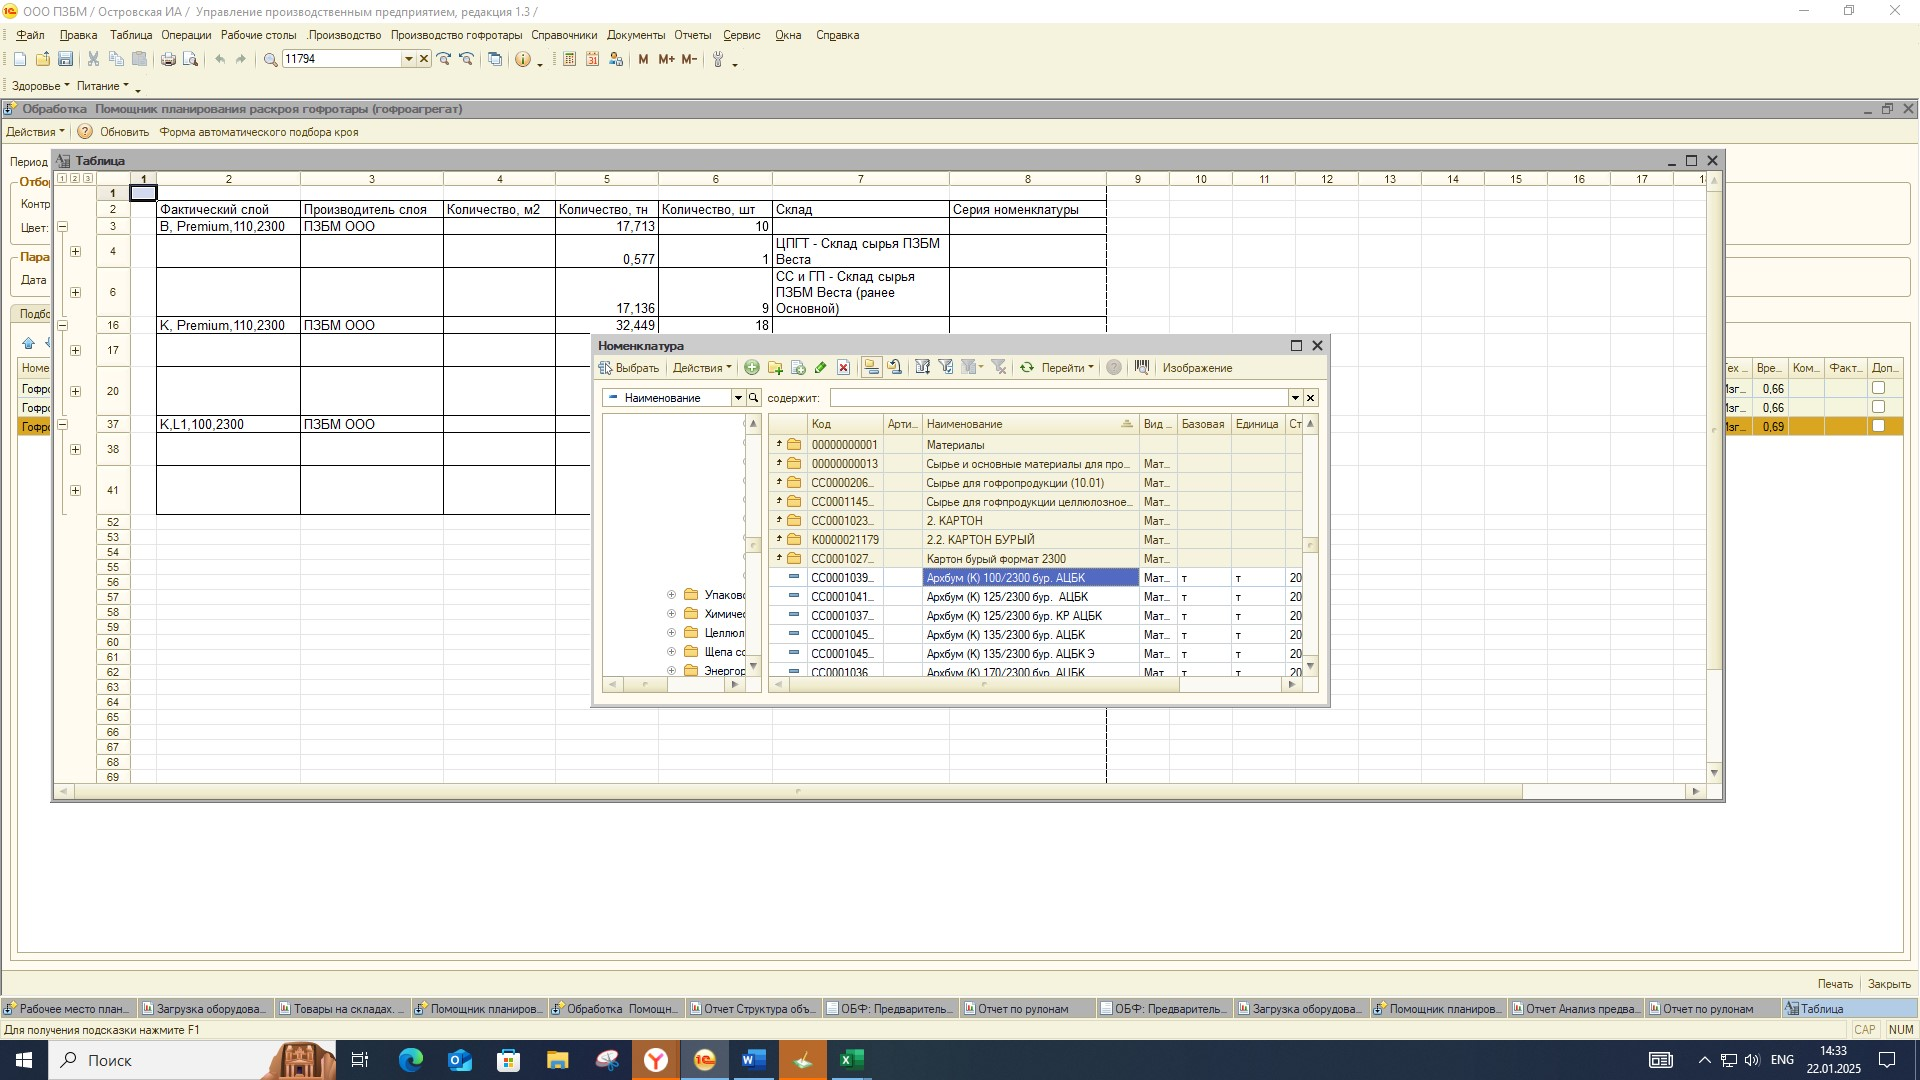
\includegraphics[height=0.35\textheight, keepaspectratio]{Pics/ПЛ10.jpg}
\end{center}
 \caption{Выбор номенклатуры слоя в композиции для раскроя}
 \label{pic:ПЛ10}
\end{figure}


\begin{figure}
\begin{center}
 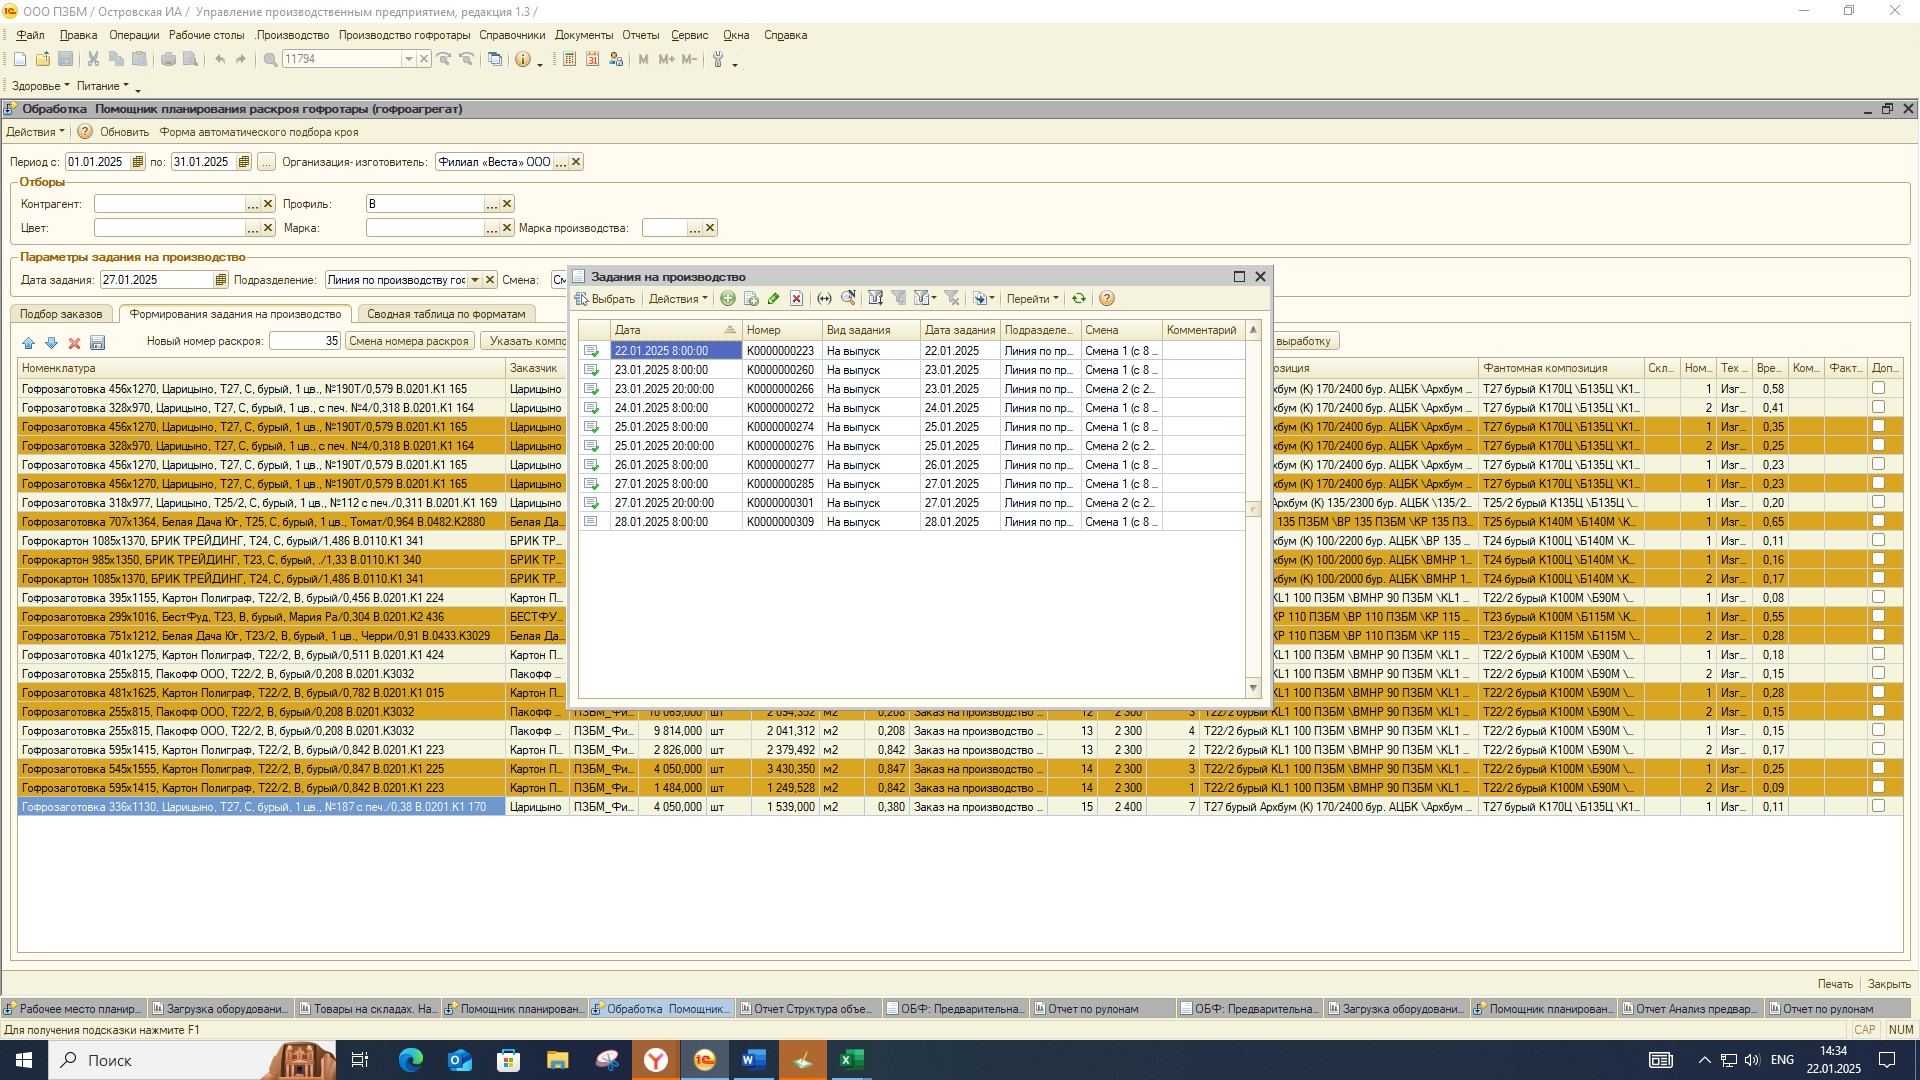
\includegraphics[height=0.35\textheight, keepaspectratio]{Pics/ПЛ11.jpg}
\end{center}
 \caption{Количество сменных заданий на производство на ГА}
 \label{pic:ПЛ11}
\end{figure}

\begin{figure}
\begin{center}
 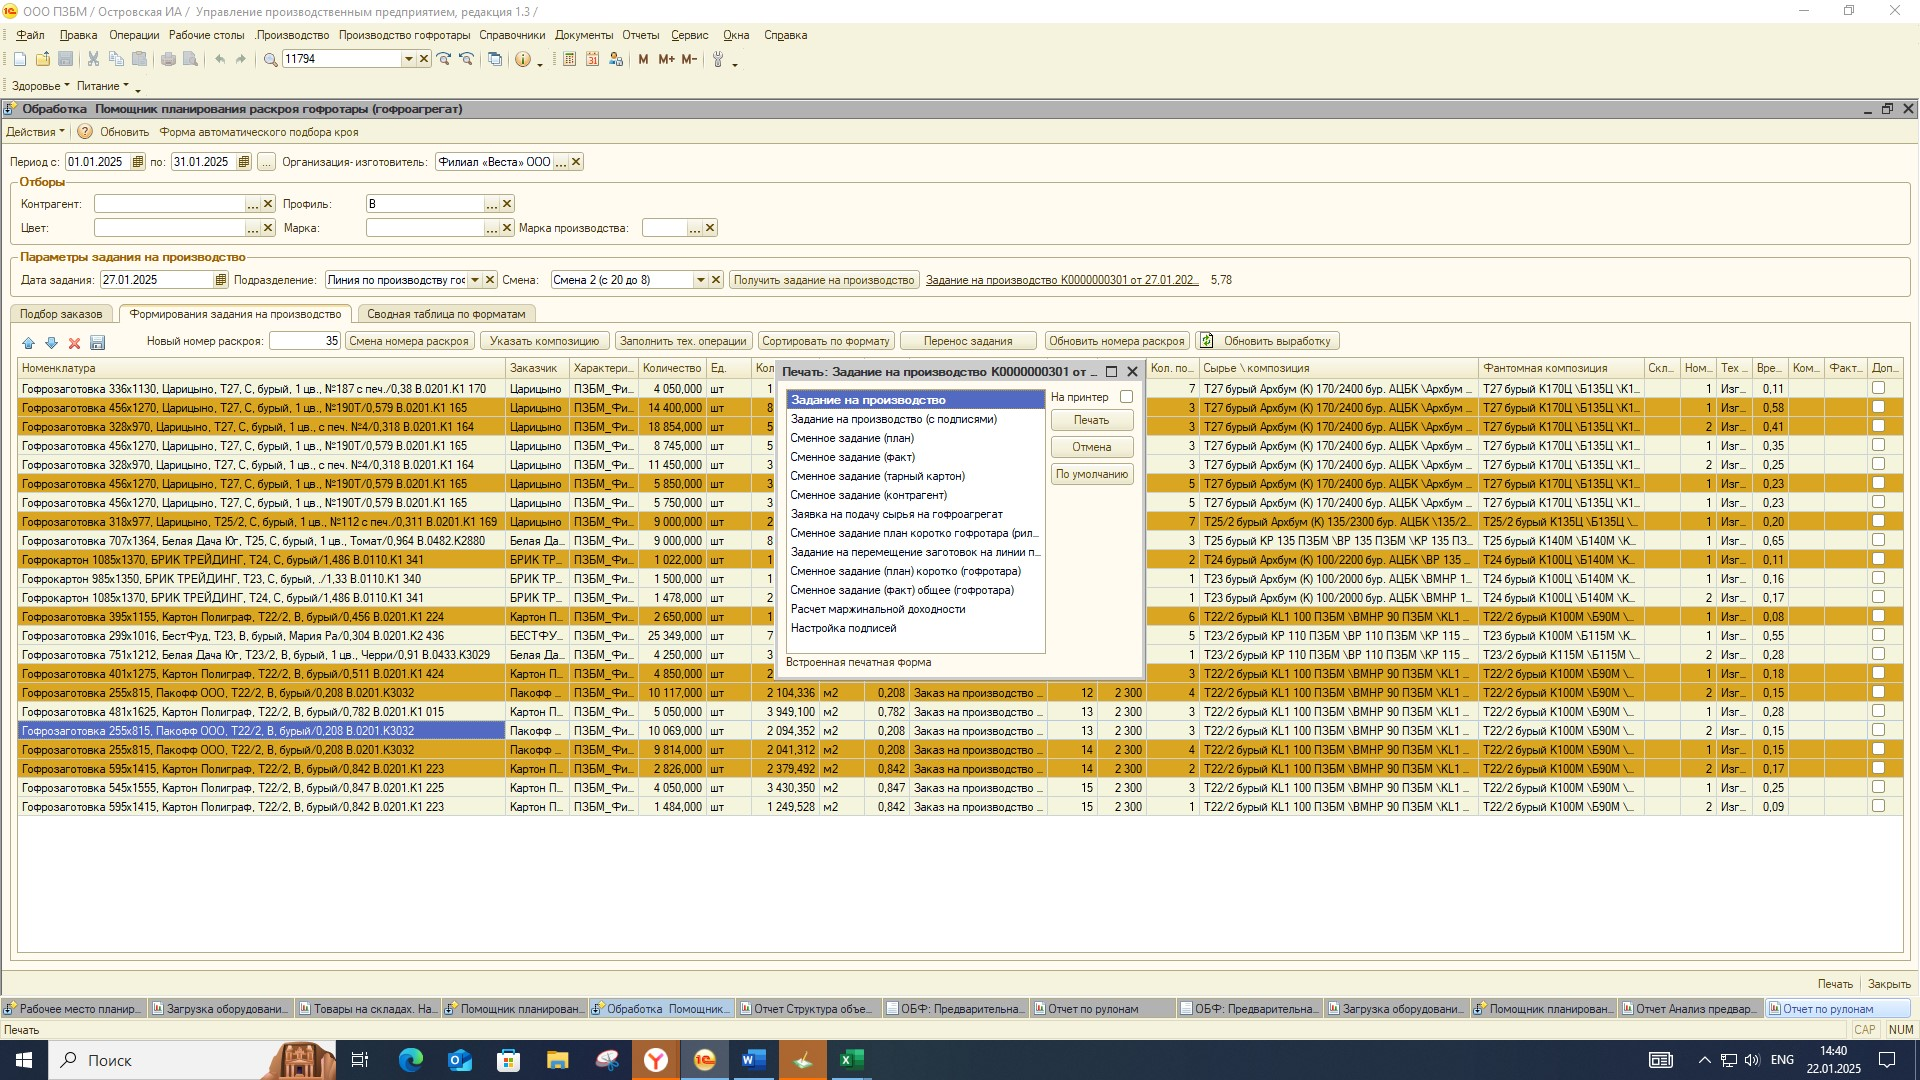
\includegraphics[height=0.35\textheight, keepaspectratio]{Pics/ПЛ12.jpg}
\end{center}
 \caption{Отправка на печать задание на производство для ГА}
 \label{pic:ПЛ12}
\end{figure}



%\begin{figure}
%\begin{center}
% 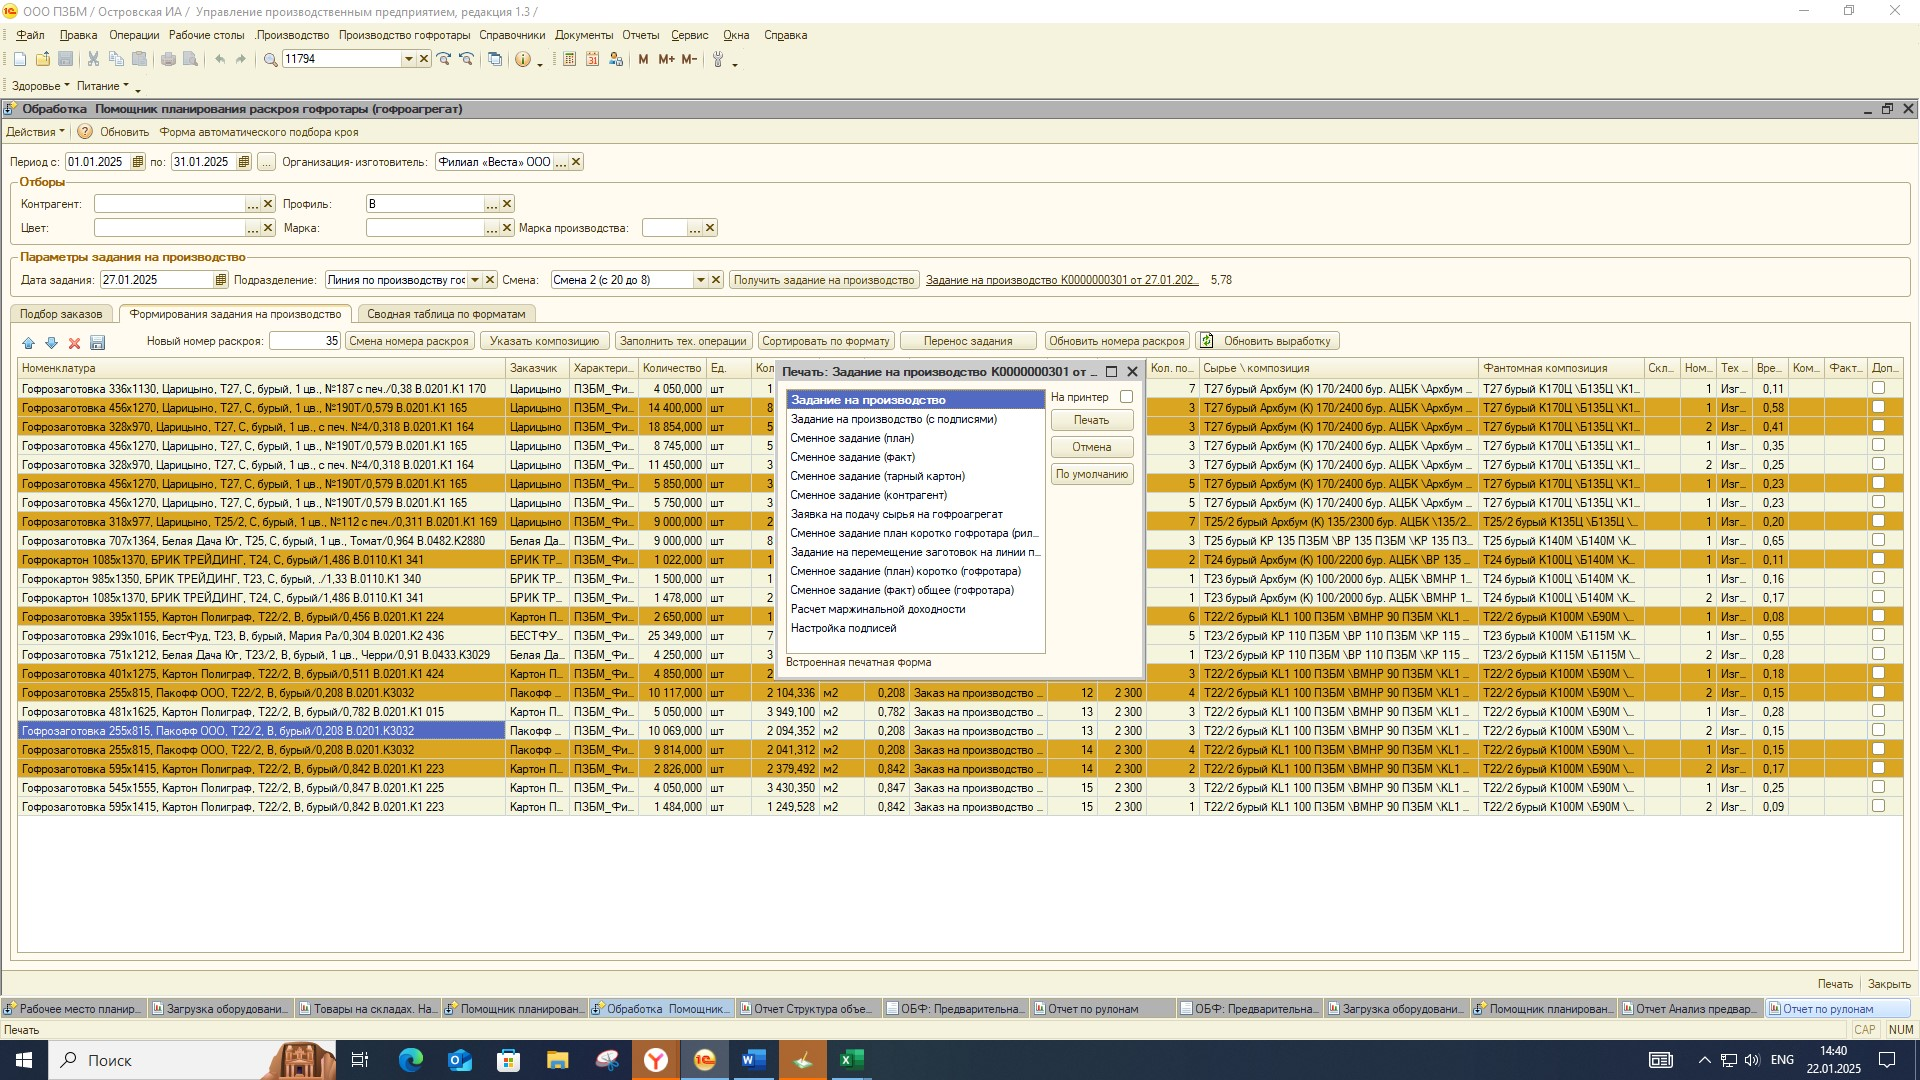
\includegraphics[height=0.35\textheight, keepaspectratio]{Pics/ПЛ12.jpg}
%\end{center}
% \caption{Отправка на печать задание на производство для ГАа}
% \label{pic:ПЛ12}
%\end{figure}

\begin{figure}
\begin{center}
 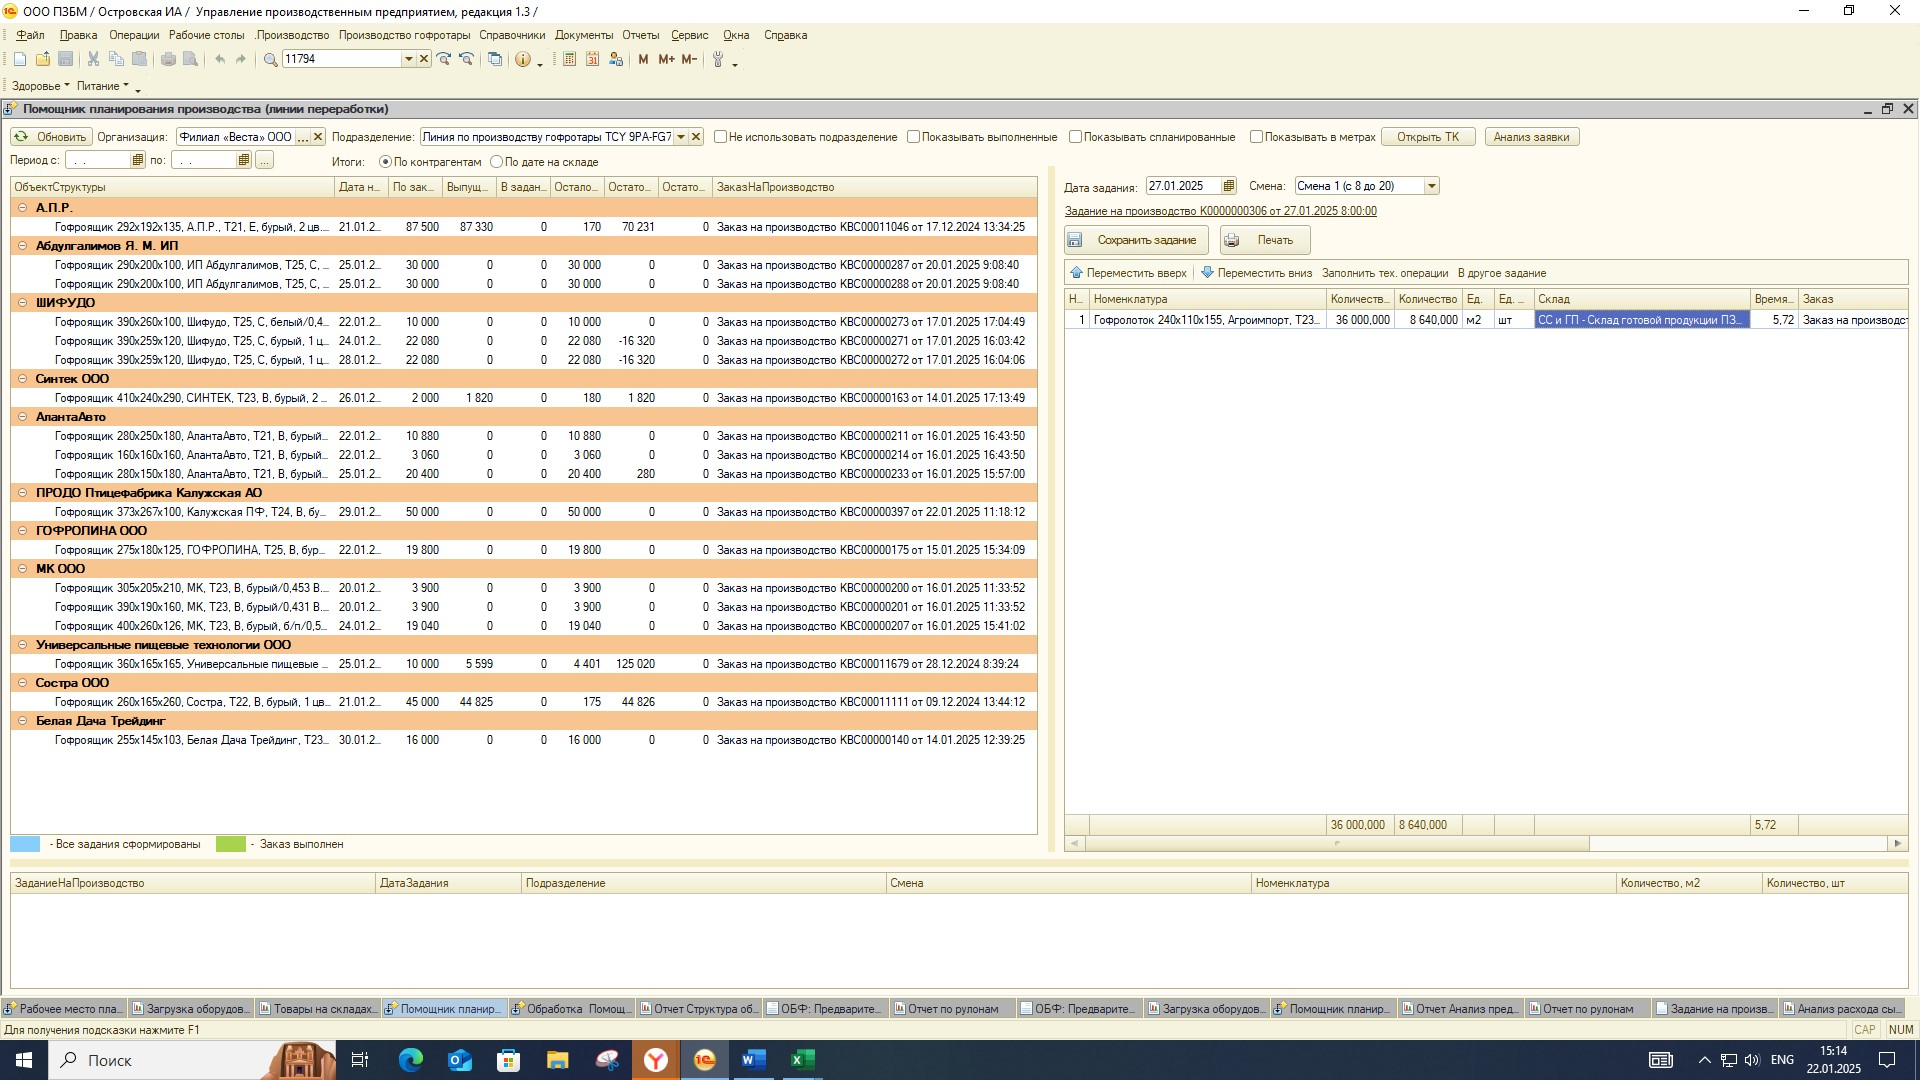
\includegraphics[height=0.45\textheight, angle=90, keepaspectratio]{Pics/ПЛ14.jpg}
\end{center}
 \caption{Планирование работы линии переработки}
 \label{pic:ПЛ14}
\end{figure}


\begin{figure}
\begin{center}
 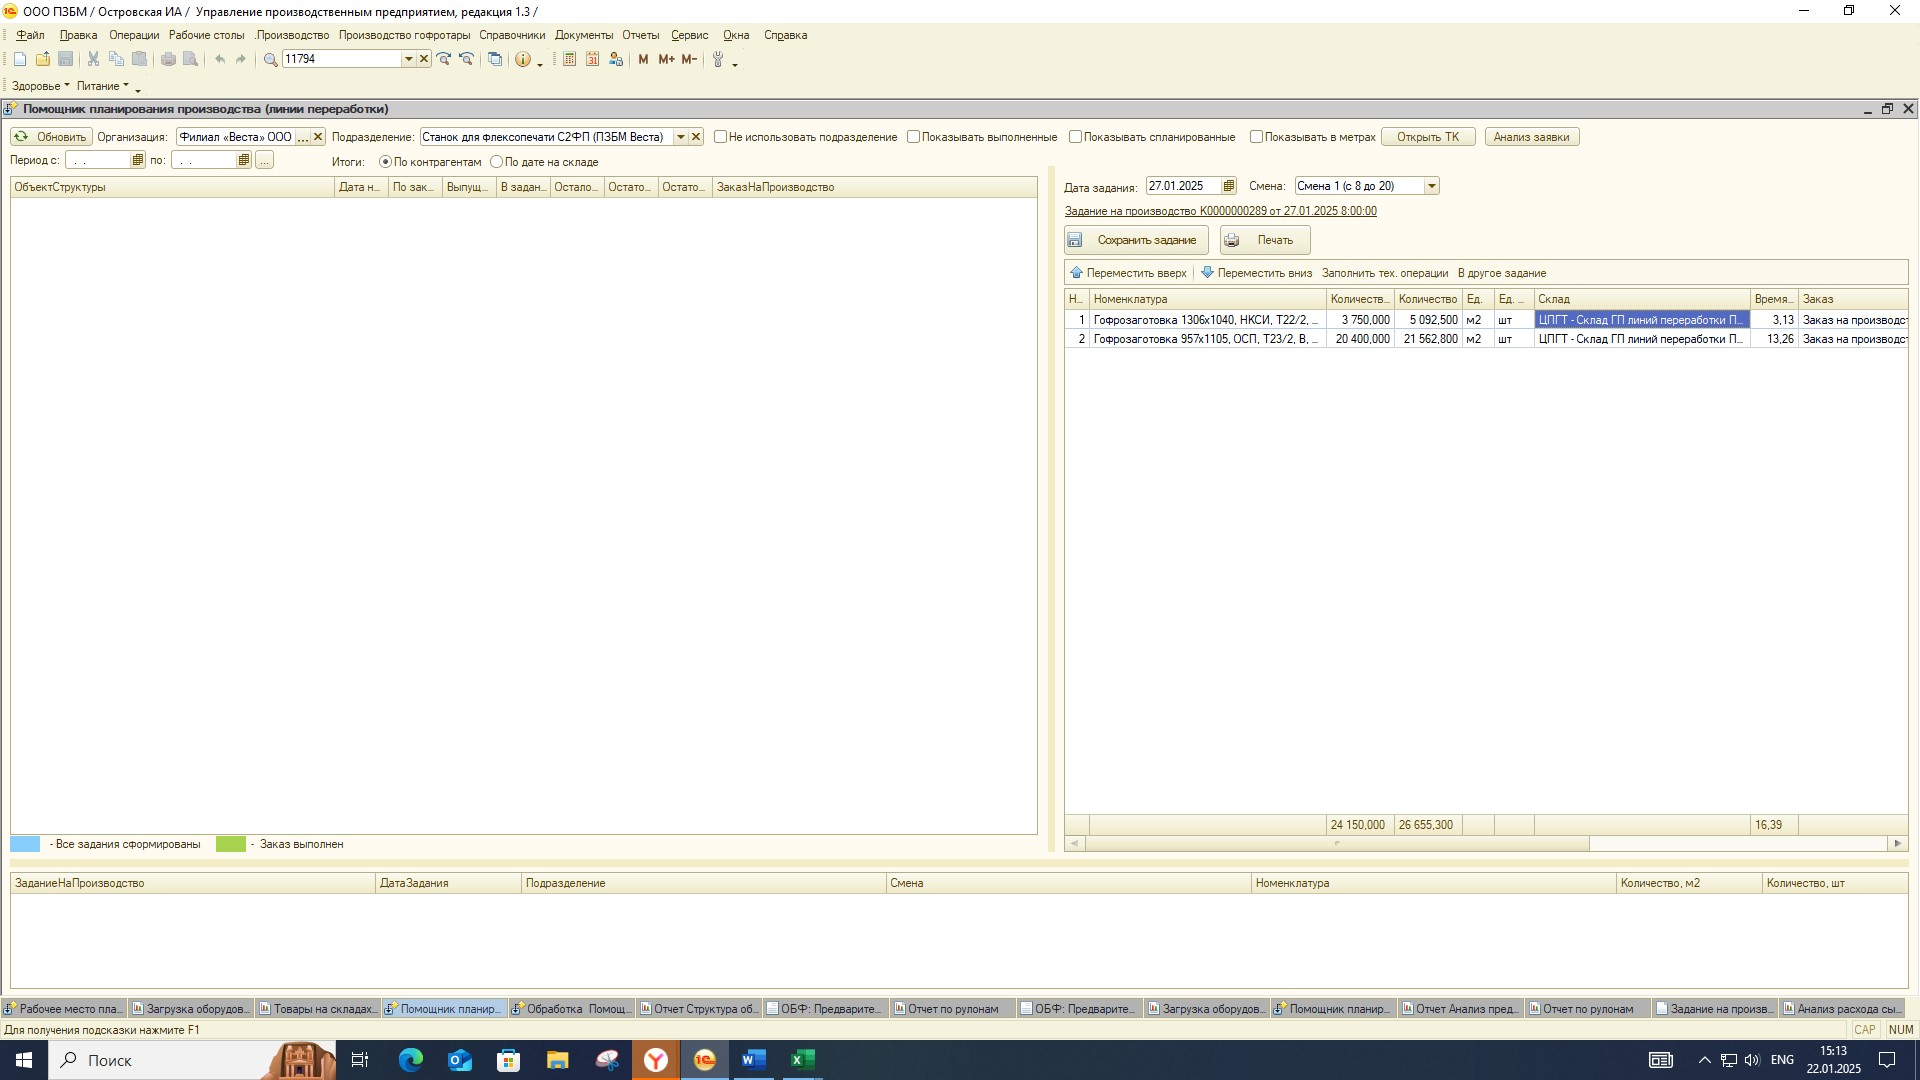
\includegraphics[height=0.35\textheight, keepaspectratio]{Pics/ПЛ13.jpg}
\end{center}
 \caption{Планировании работы линии переработки с учетом простоя}
 \label{pic:ПЛ13}
\end{figure}

\clearpage
% Все заявки от покупателей  менеджеры отдела продаж регистрируют в системе СБИС.

% Менеджер выгружает в отдел планирования в системе СБИС заявки покупателей. 
% Отдел БППП формирует список заказов из системы СБИС. Менеджер должен завести заявки клиентов до 15.00 рабочего дня. Заявки, заведенные после этого времени, будут переведены на следующий день. Инженер БППП ориентируется на желаемую дату производства, которую указал менеджер. 
% Инженер в системе СБИС выгружает заявки в систему планирования PMASC. 
% Система СБИС выгружает заявку полностью. В заявке может быть несколько строк (заказов). В систему PMASC заявка загружается с номером СБИС, номер заказа указывается как номер заявки СБИС + номер строки в заявке.
% Менеджеры могут прикрепить в СБИС файлы с макетами и оснасткой.


% Система PMASC позволяет для загруженных заявок сформировать оптимальные схемы раскроя гофрополотна по заданным параметрам.
% В системе по умолчанию инженер БППП указывает дату между заказами в раскрое 1 день. Это позволяет кроить заказы, которые менеджеры поставили в один желаемый день производства. Крой выполняется по марке. Оперативные остатки по сырью (бумага и картон) инженер БППП получает из системы СБИС (рис. \ref{pic:d6}).   

% В ходе обследования выявлены нормативные марки и состав композиций  (рис. \ref{pic:d7}).  
% Нормативы по композициям устаревшие и требуют обновления.
% Далее инженер БППП в системе PMASC выполняет автоматический поиск раскроев, редактирует список раскроев и подбирает композиции сырья вручную. 
% Сохраненные и принятые в работу раскрои инженер БППП экспортирует из системы
%  PMASC в систему СБИС через файлы обмена формата xml. 
% Загруженные раскрои в системе СБИС находятся в журнале раскроев (рис. \ref{pic:d7}). 
% В системе СБИС есть возможность смотреть план, но менеджеры не используют эту возможность, потому как нужно переключать модуль в виду отсутствия возможности работы одновременно в разных режимах.

% Инженер БППП печатает крой (рис. \ref{pic:dd10}) в количестве 9 экземпляров.
% Задание (крой) передается в коммерческий отдел для планирования производства.
% Менеджеры коммерческого отдела выбирают в заданиях в крой те заказы, которые нужно брать в работу с учетом желаемой даты производства.
% Раскрои с датами заместитель директора по производству возвращает от менеджеров в БППП.
% Заместитель директора по производству указывает композицию сырья в раскроях по плану и передает задание на гофроагрегат в цех, через мастера производства.


% Планирование линий переработки

% Каждый день инженер БППП создает отчет по заготовкам, выпущенным с гофроагрегата (рис. \ref{pic:d14}) вручную. 
% Инженер БППП в системе PMASC создает план на переработку вручную: план на ящики, отдельно план на сложную высечку, отдельно план на изготовление решетки и прокладки.
% Инженер БППП печатает задание на линию из системы PMASC (рис. \ref{pic:d15}) и передает мастеру производства. 
% Мастер производства при получении плана работы самостоятельно распределяет задания по линиям исходя из загруженности линий, возможности производства.
% Задания передаются операторам линий переработки. 





% %\todo{Добавить планирование в плановом отделе, планирование линий}

% %Также на основании рапортов с производства планировщик ведет отчеты в таблицах MS Excel на сервере: 
% %\begin{enumerate}
% %     \item Отчет по %производству за период (рис. \ref{pic:pic_a23}).
% %     \item Отчет по %выработке ГА и линий (рис. \ref{pic:pic_a24}).
% %     \item Отчет по %простоям (рис. \ref{pic:pic_a25}).
% % \end{enumerate}

% %Кто-то??? распечатывает ярлыки на товарный картон (Кто?). 


% % \begin{figure}
% % \begin{center}
% %   
\includegraphics[height=0.8\textheight, width=0.94\textwidth, keepaspectratio]{Pics/Pattern.jpg}
% % \end{center}
% %   \caption{Заявка на приобретение продукции}
% %   \label{pic:d16}
% % \end{figure}
% % % \clearpage

% \begin{figure}
% \begin{center}
%   \includegraphics[height=0.8\textheight, width=0.94\textwidth, keepaspectratio]{Pics/d6.jpg}
% \end{center}
%   \caption{Остатки по рулонам}
%   \label{pic:d6}
% \end{figure}

% \begin{figure}
% \begin{center}
%   \includegraphics[height=0.8\textheight, width=0.94\textwidth, keepaspectratio]{Pics/d7.jpg}
% \end{center}
%   \caption{Принятые композиции по сырью}
%   \label{pic:d7}
% \end{figure}

% \begin{figure}
% \begin{center}
%   \includegraphics[height=0.8\textheight, width=0.94\textwidth, keepaspectratio]{Pics/dd10.jpg}
% \end{center}
%   \caption{Раскрои гофрокартона}
%   \label{pic:dd10}
% \end{figure}

% \begin{figure}
% \begin{center}
%   \includegraphics[height=0.8\textheight, width=0.94\textwidth, keepaspectratio]{Pics/d15.jpg}
% \end{center}
%   \caption{Задание на линию из системы PMASC}
%   \label{pic:d15}
% \end{figure}

% \begin{figure}
% \begin{center}
%   \includegraphics[height=0.8\textheight, width=0.94\textwidth, keepaspectratio]{Pics/d14.jpg}
% \end{center}
%   \caption{Отчет по заготовкам с ГА}
%   \label{pic:d14}
% \end{figure}

% \clearpage

% \ifx \notincludehead\undefined
\normalsize
\end{document}
\fi